%part3.tex

\part{\LaTeX{} 图形命令的使用}

\section{水平间距和居中}\label{sec:center}

\subsection{水平居中}\label{ssec:hcenter}
图形的放置位置由当前文本的排列方式所决定。
为使图形居中放置,可将其放入居中环境 \env{center} 中。
\begin{lstlisting}
\begin{center}
\includegraphics[width=2in]{graphic.eps}
\end{center}
\end{lstlisting}

如果 \cmd{includegraphics} 命令处于一个环境中
(例如 \env{minipage} 或 \env{figure}),
用 \cmdi{centering} 可将其后的内容居中排列。
例如:

\begin{lstlisting}
\begin{figure}
\centering
\includegraphics[width=2in]{graphic.eps}
\end{figure}
\end{lstlisting}
效果类似于
\begin{lstlisting}
\begin{figure}
\begin{center}
\includegraphics[width=2in]{graphic.eps}
\end{center}
\end{figure}
\end{lstlisting}
这里推荐使用~\cmd{centering},因为~\verb+\begin{center}+~会使图形上下
方的垂直间距增加一倍
( \env{figure} 带有的垂直间距加上 \env{center} 环境带有的垂直间距)。
若希望有额外的垂直间距,可使用第~\ref{ssec:vspace}~节介绍的命令。

\cmd{psfig} 和 \cmd{epsfbox} 命令
\marginpar{过时的用法}
的缺陷让它们很难使图形居中排列。
过去,作为一种解决办法,使用了 \TeX{} 命令 \cmdi{centerline} 和 \cmdi{leavevmode}。
而 \cmd{includegraphics} 命令已克服了这些缺陷,
允许直接与 \cmd{centering} 命令一起使用或用在 \env{center} 环境中,
因此也就不需再使 \cmd{centerline} 和 \cmd{leavevmode}了。

\subsection{水平间距}\label{ssec:hspace}
\LaTeX{} 在排列图形的时候实际上与排列其它的像文字这样的对象是一样的,
了解到这一点很重要。
举例来说,如果行尾不是以 \texttt{\%} 结束的话,
\LaTeX{} 会自动在两行之间加进一个字符的水平间距。
例如,
\begin{lstlisting}
Hello
World
\end{lstlisting}
在输出结果中``Hello'' 和 ``World'' 之间会有一个字符的水平间距。
类似地,
\begin{lstlisting}
\includegraphics{file}
\includegraphics{file}
\end{lstlisting}
则在图形之间有一个字符的水平间距。
在第一行的行尾加上注释符\texttt{\%}
\begin{lstlisting}
\includegraphics{file}%
\includegraphics{file}
\end{lstlisting}
就会取消图形之间的水平间距。

如果需要水平间距,可用 \cmdi{hspace} 命令在图形之间
加入指定长度
\footnote{
	用 \cmd{textwidth} 或 \texttt{em} (原文误作 \cmd{em}——译者注)等作为 \cmd{hspace} 的参数,
	而不是采用固定长度,可提高文档的通用性。}
或用 \cmdi{hfill} 加入一个可填充可能的间距的弹性长度。
例如:
\begin{lstlisting}
\includegraphics{file.eps}\hfill\includegraphics{file.eps}
\end{lstlisting}
将两个图形尽量向左右分开。而
\begin{lstlisting}
\hspace*{\fill}\includegraphics{file.eps}%
\hfill\includegraphics{file.eps}\hspace*{\fill}
\end{lstlisting}
使得图形的两边和中间的间距都相等。
由于断行前的 \cmd{hfill} 命令会被忽略,
所以需要用\cmdonearg{hspace*}{\cmd{fill}} 来替代它。

除了 \cmd{hspace} 和 \cmd{hfill} 之外,
\marginpar{其它间距命令}
\cmdi{quad} 命令会插入当前字体大小的空白。
例如,如果使用 \texttt{10 pt} 字体大小,那么 \cmd{quad} 会插入 10 \texttt{pt} 的水平间距。
而命令 \cmdi{qquad} 会插入两倍于 \cmd{quad} 的水平间距。


\section{旋转、缩放和对齐}\label{sec:rotate-scale-align}

\subsection{高度和整体高度的区别}\label{ssec:diffheight}

使用 \opt{height} 选项时必须要小心,
因为用户经常想要的其实是由 \opt{totalheight} 选项设置的整体高度
(参见~\pageref{fig:samplebox} 页的图~\ref{fig:samplebox})。
当对象的深度为零时,对象的整体高度就是它的高度,
此时使用 \opt{height} 选项不会有什么问题。
但是,当对象的深度不为零时,使用 \opt{height} 而不是 \opt{totalheight} 会导致不正确的图像大小或除零的错误。
导入图像时,区分 \opt{height} 和 \opt{totalheight} 对于旋转和缩放时显得尤其重要。
例如:
\begin{lstlisting}
\includegraphics[angle=-45,totalheight=1in]{file}
\includegraphics[angle=-45,height=1in]{file}
\end{lstlisting}
第一个命令缩放一个旋转了的图形,使其全部高度为~1~英寸。
而第二个命令缩放一个旋转了的图形,使其在参考点以上的部分为~1~英寸高。

\subsection{旋转图形的缩放}\label{ssec:enlarge}
当在插图命令中指定高度或宽度时,这里给出的大小并不是图形的大小,
而是图形的 BoundingBox 的大小。
这点在图形旋转和缩放时很重要。例如:
\begin{lstlisting}
\begin{center}
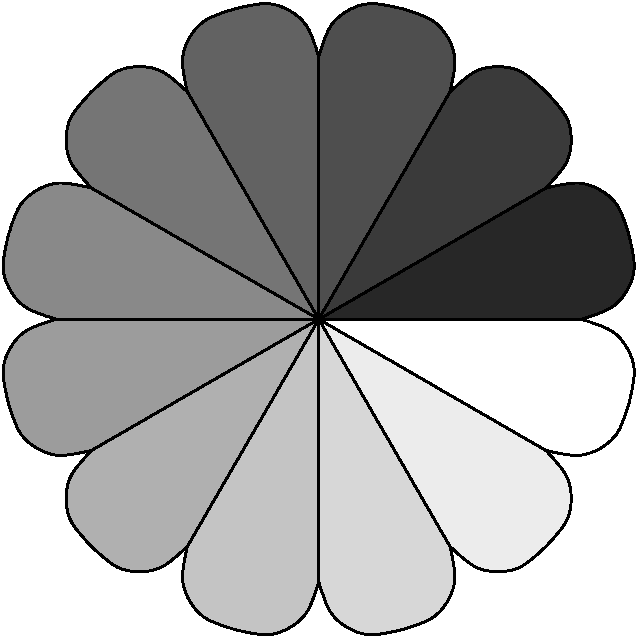
\includegraphics[totalheight=1in]{rosette}
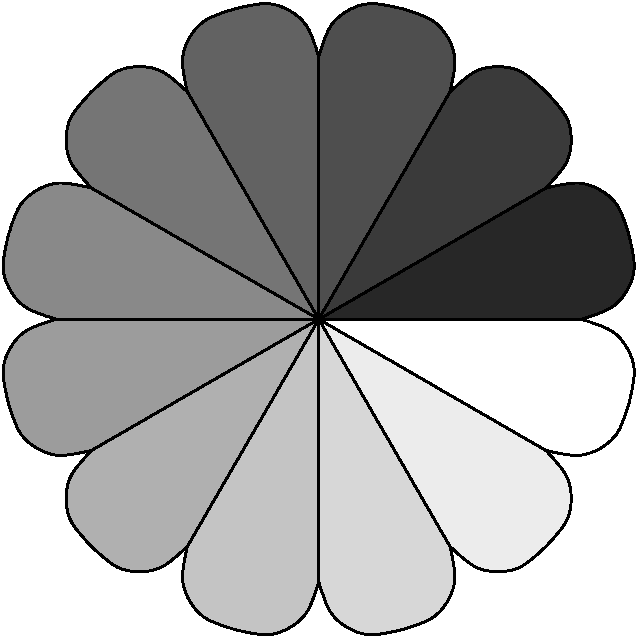
\includegraphics[angle=45,totalheight=1in]{rosette}
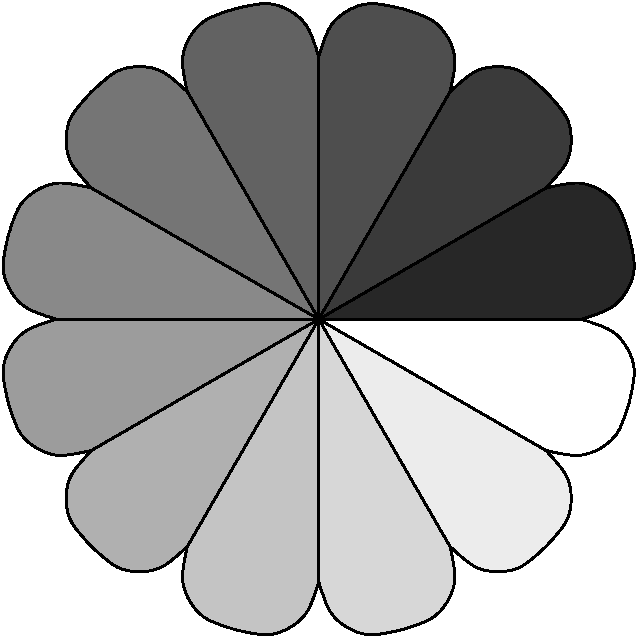
\includegraphics[angle=90,totalheight=1in]{rosette}
\end{center}
\end{lstlisting}
得到

\begin{center}
	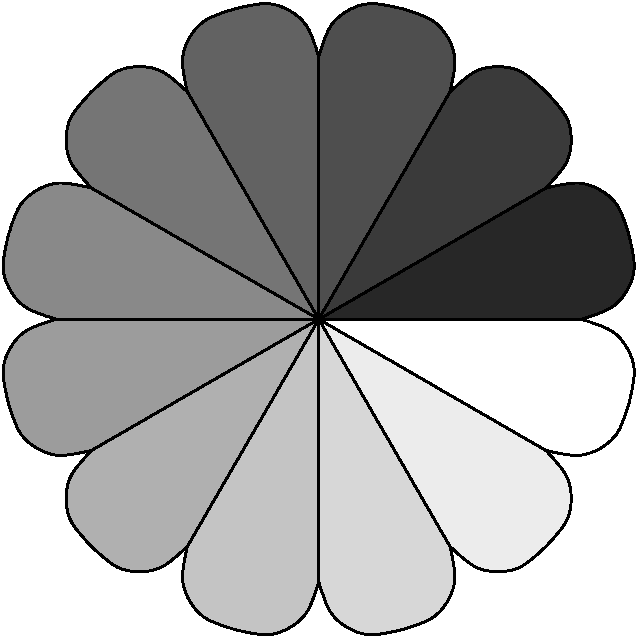
\includegraphics[totalheight=1in]{rosette}
	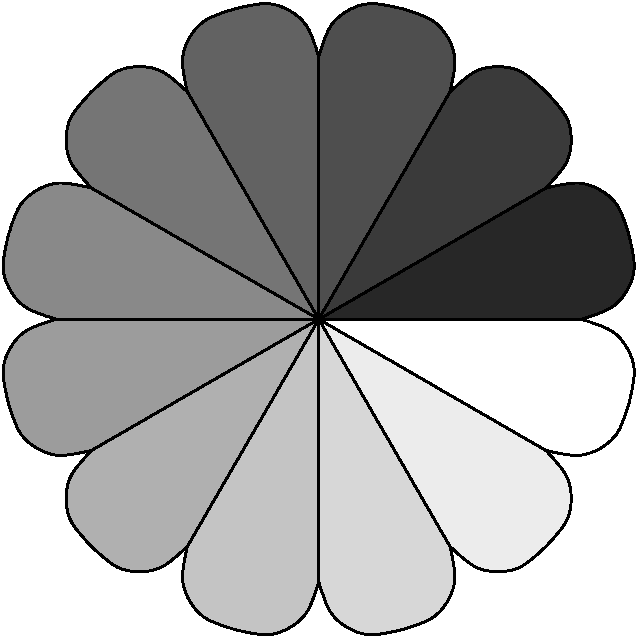
\includegraphics[angle=45,totalheight=1in]{rosette}
	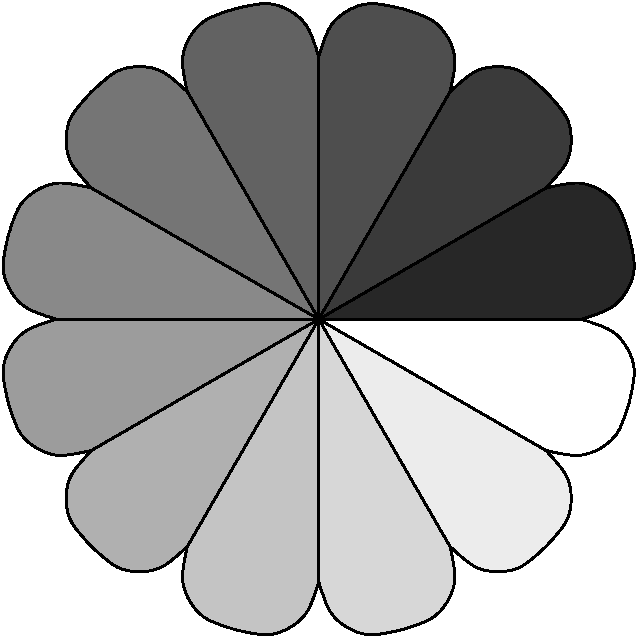
\includegraphics[angle=90,totalheight=1in]{rosette}
\end{center}
尽管看上去图形的大小不一有点奇怪,
但在看过它们的~BoundingBox~后就会明白了。

\begin{center}
	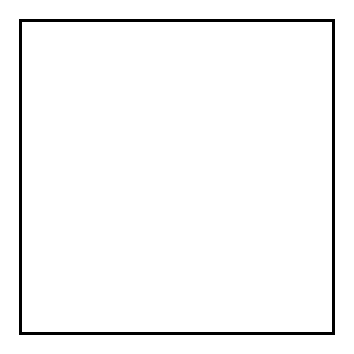
\includegraphics[totalheight=1in]{rosettebox}
	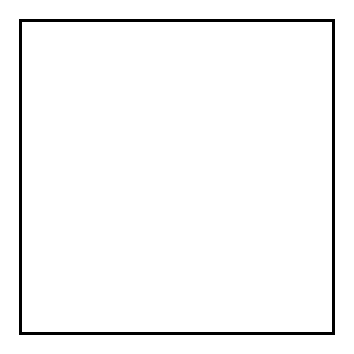
\includegraphics[angle=45,totalheight=1in]{rosettebox}
	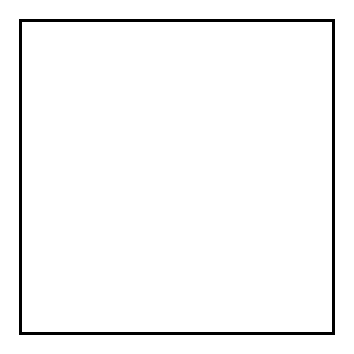
\includegraphics[angle=90,totalheight=1in]{rosettebox}
\end{center}
每一幅图像的结果是旋转后的BoundingBox 为1英寸高。
缩放功能改变的是BoundingBox 的大小,而不是实际看到图像的大小。


\subsection{旋转图形的对齐}\label{ssec:ralign}

\subsubsection{第一个例子}

当图形被旋转时,可能会出现不对齐的情况。例如:

\begin{lstlisting}
\begin{center}
   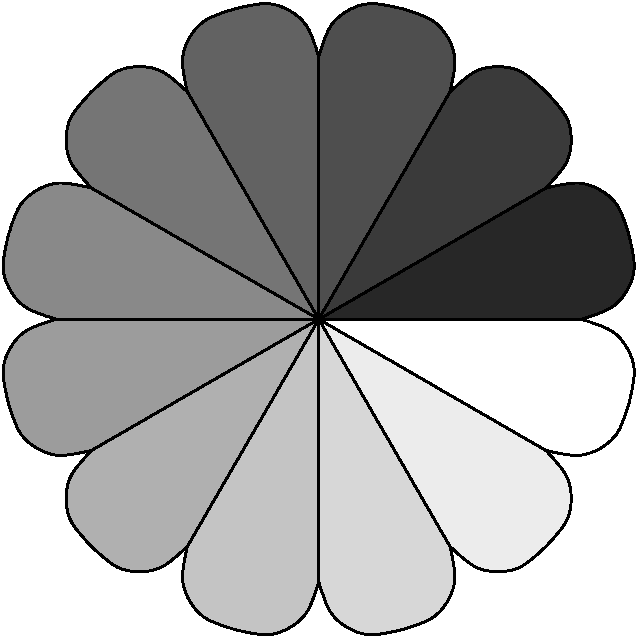
\includegraphics[totalheight=1in]{rosette}
   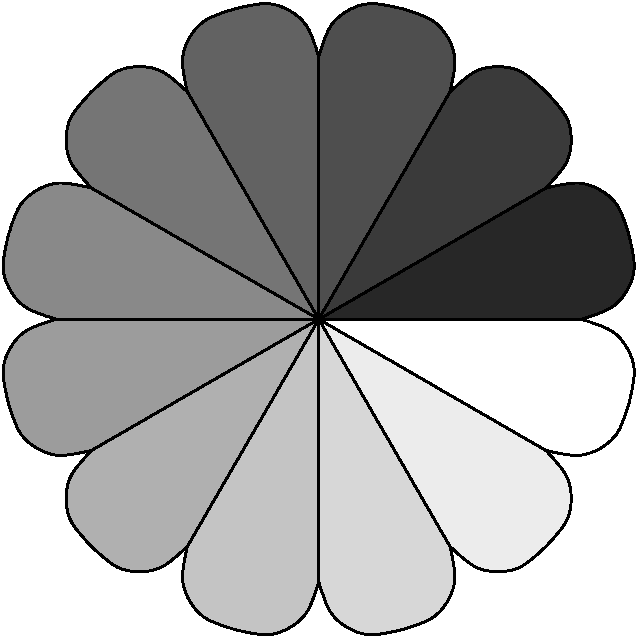
\includegraphics[totalheight=1in,angle=-45]{rosette}
   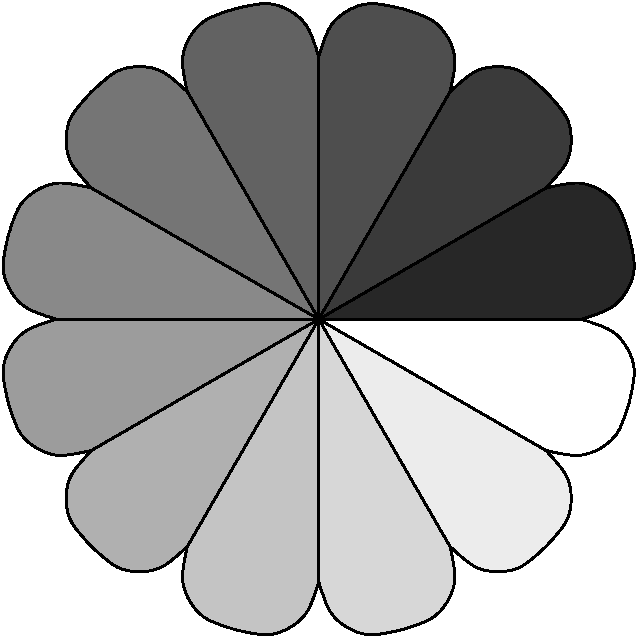
\includegraphics[totalheight=1in,angle=-90]{rosette}
\end{center}
\end{lstlisting}
得到

\begin{center}
   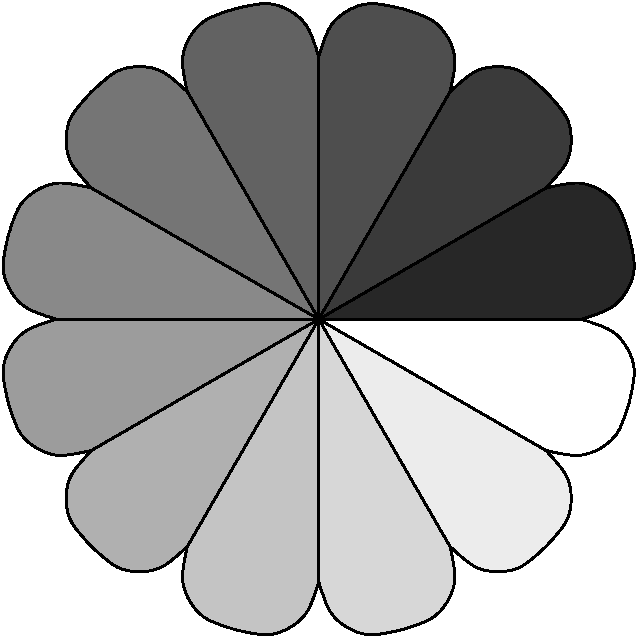
\includegraphics[totalheight=1in]{rosette}
   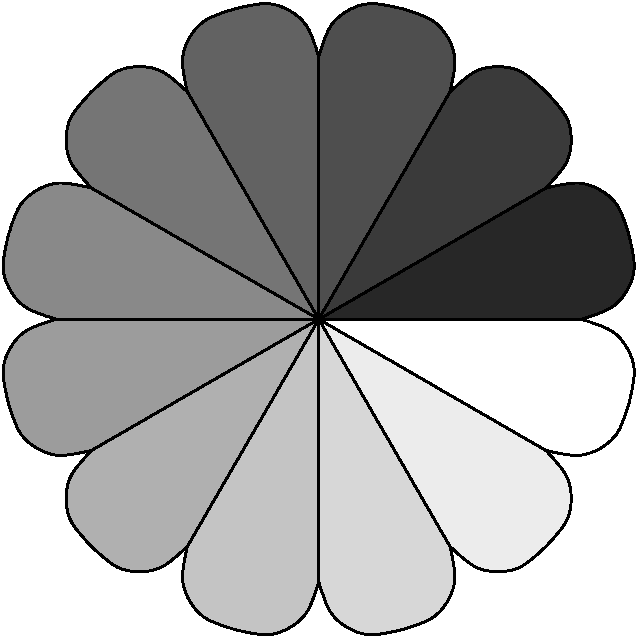
\includegraphics[totalheight=1in,angle=-45]{rosette}
   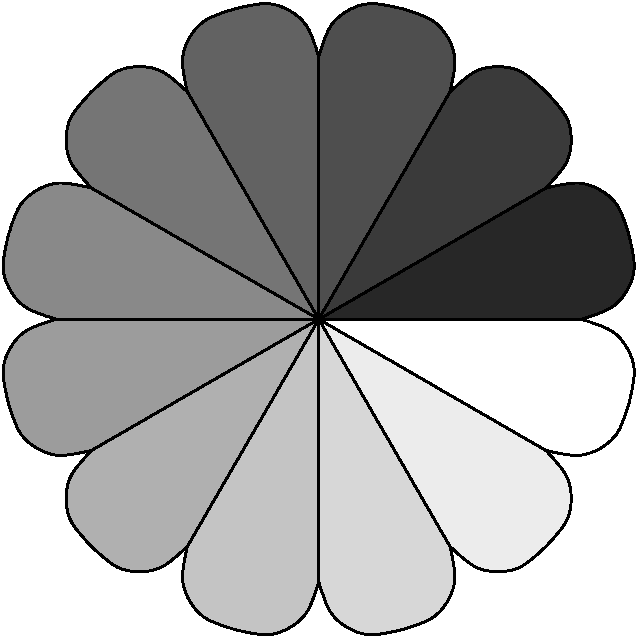
\includegraphics[totalheight=1in,angle=-90]{rosette}
\end{center}
当然,这种现象仍可用图形的~BoundingBox~来解释。

\begin{center}
   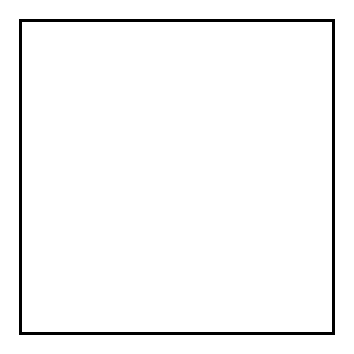
\includegraphics[totalheight=1in]{rosettebox}
   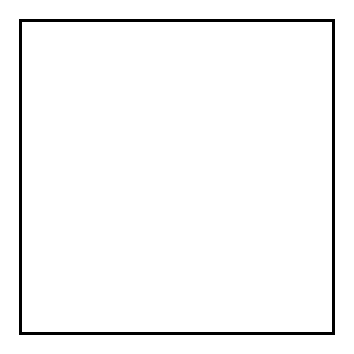
\includegraphics[totalheight=1in,angle=-45]{rosettebox}
   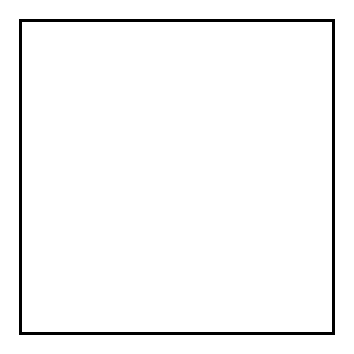
\includegraphics[totalheight=1in,angle=-90]{rosettebox}
\end{center}
在这种情况下,我们可以看到图形对象的参考点(左下角)是处于同一水平线上的。
如果希望是中间对齐,那么可以用 \cmd{includegraphics} 的 \opt{origin} 选项。
\begin{lstlisting}
\begin{center}
   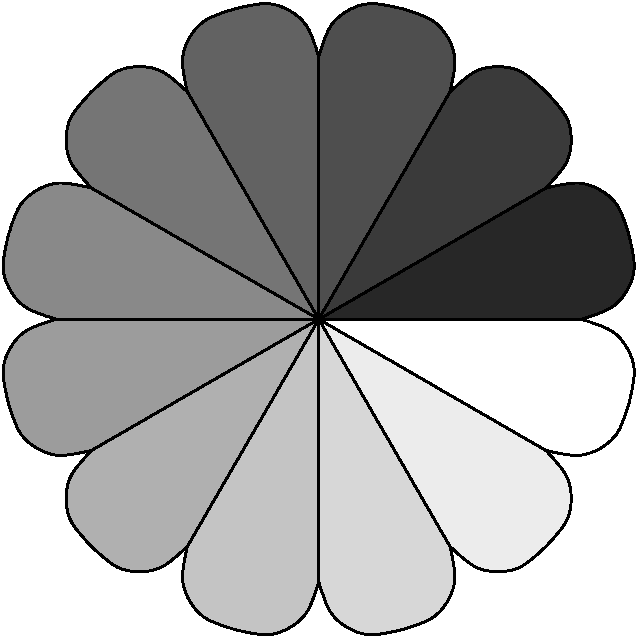
\includegraphics[totalheight=1in]{rosette}
   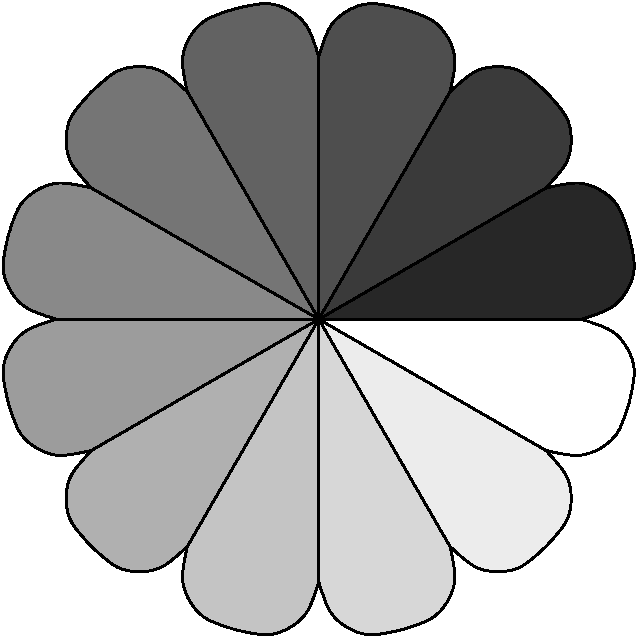
\includegraphics[totalheight=1in,origin=c,angle=-45]{rosette}
   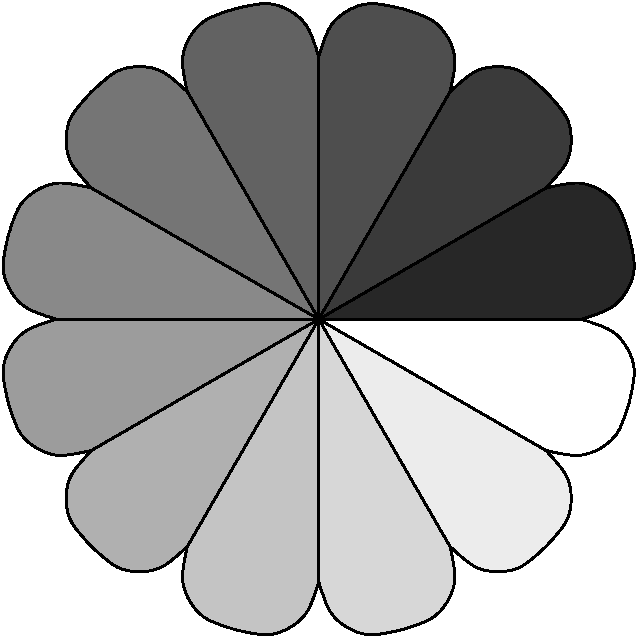
\includegraphics[totalheight=1in,origin=c,angle=-90]{rosette}
\end{center}
\end{lstlisting}
这次所有图形都是中间对齐的。

\begin{center}
   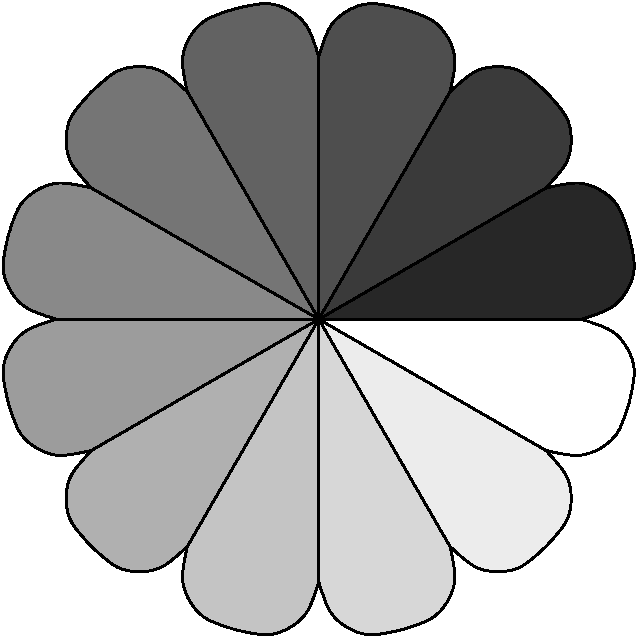
\includegraphics[totalheight=1in]{rosette}
   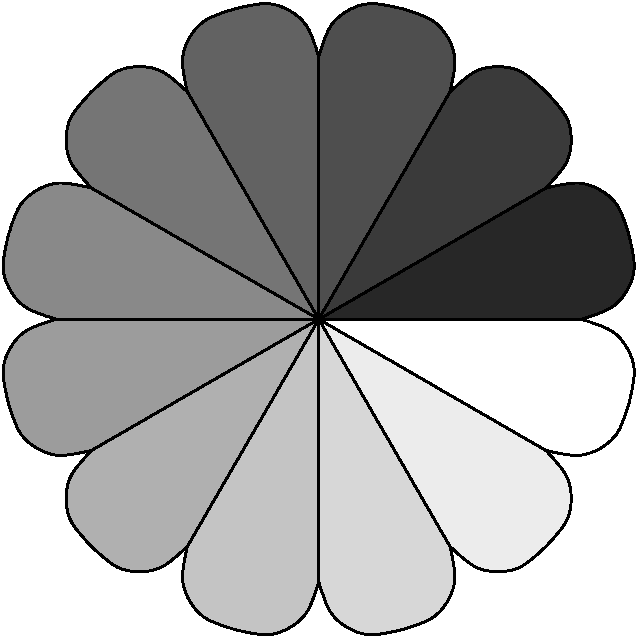
\includegraphics[totalheight=1in,origin=c,angle=-45]{rosette}
   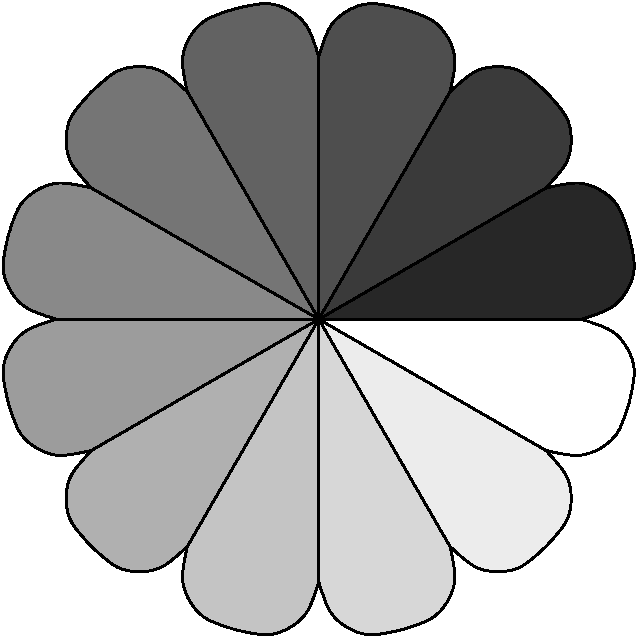
\includegraphics[totalheight=1in,origin=c,angle=-90]{rosette}
\end{center}

\subsubsection{第二个例子}
同样地,下面的命令
\begin{lstlisting}
\begin{center}
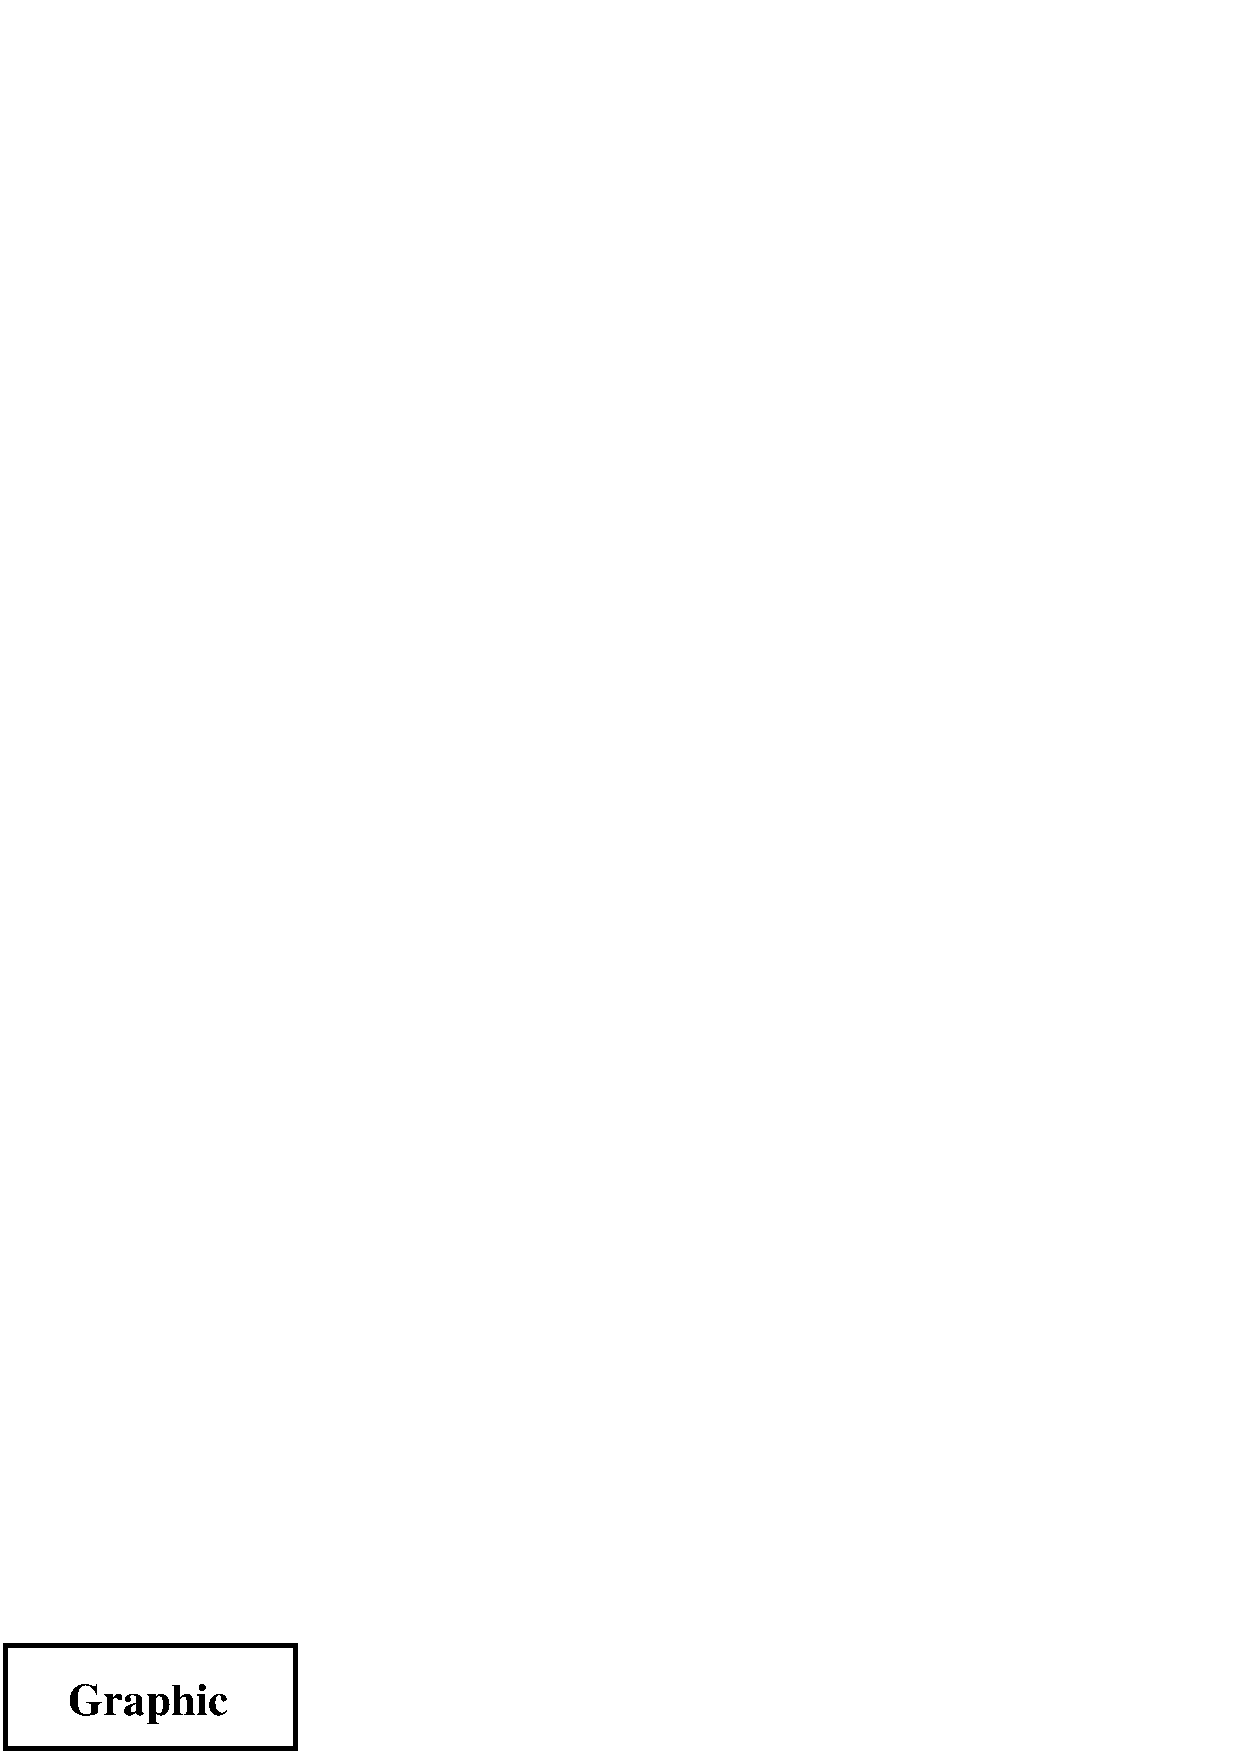
\includegraphics[width=1in]{graphic}
\hspace{1in}
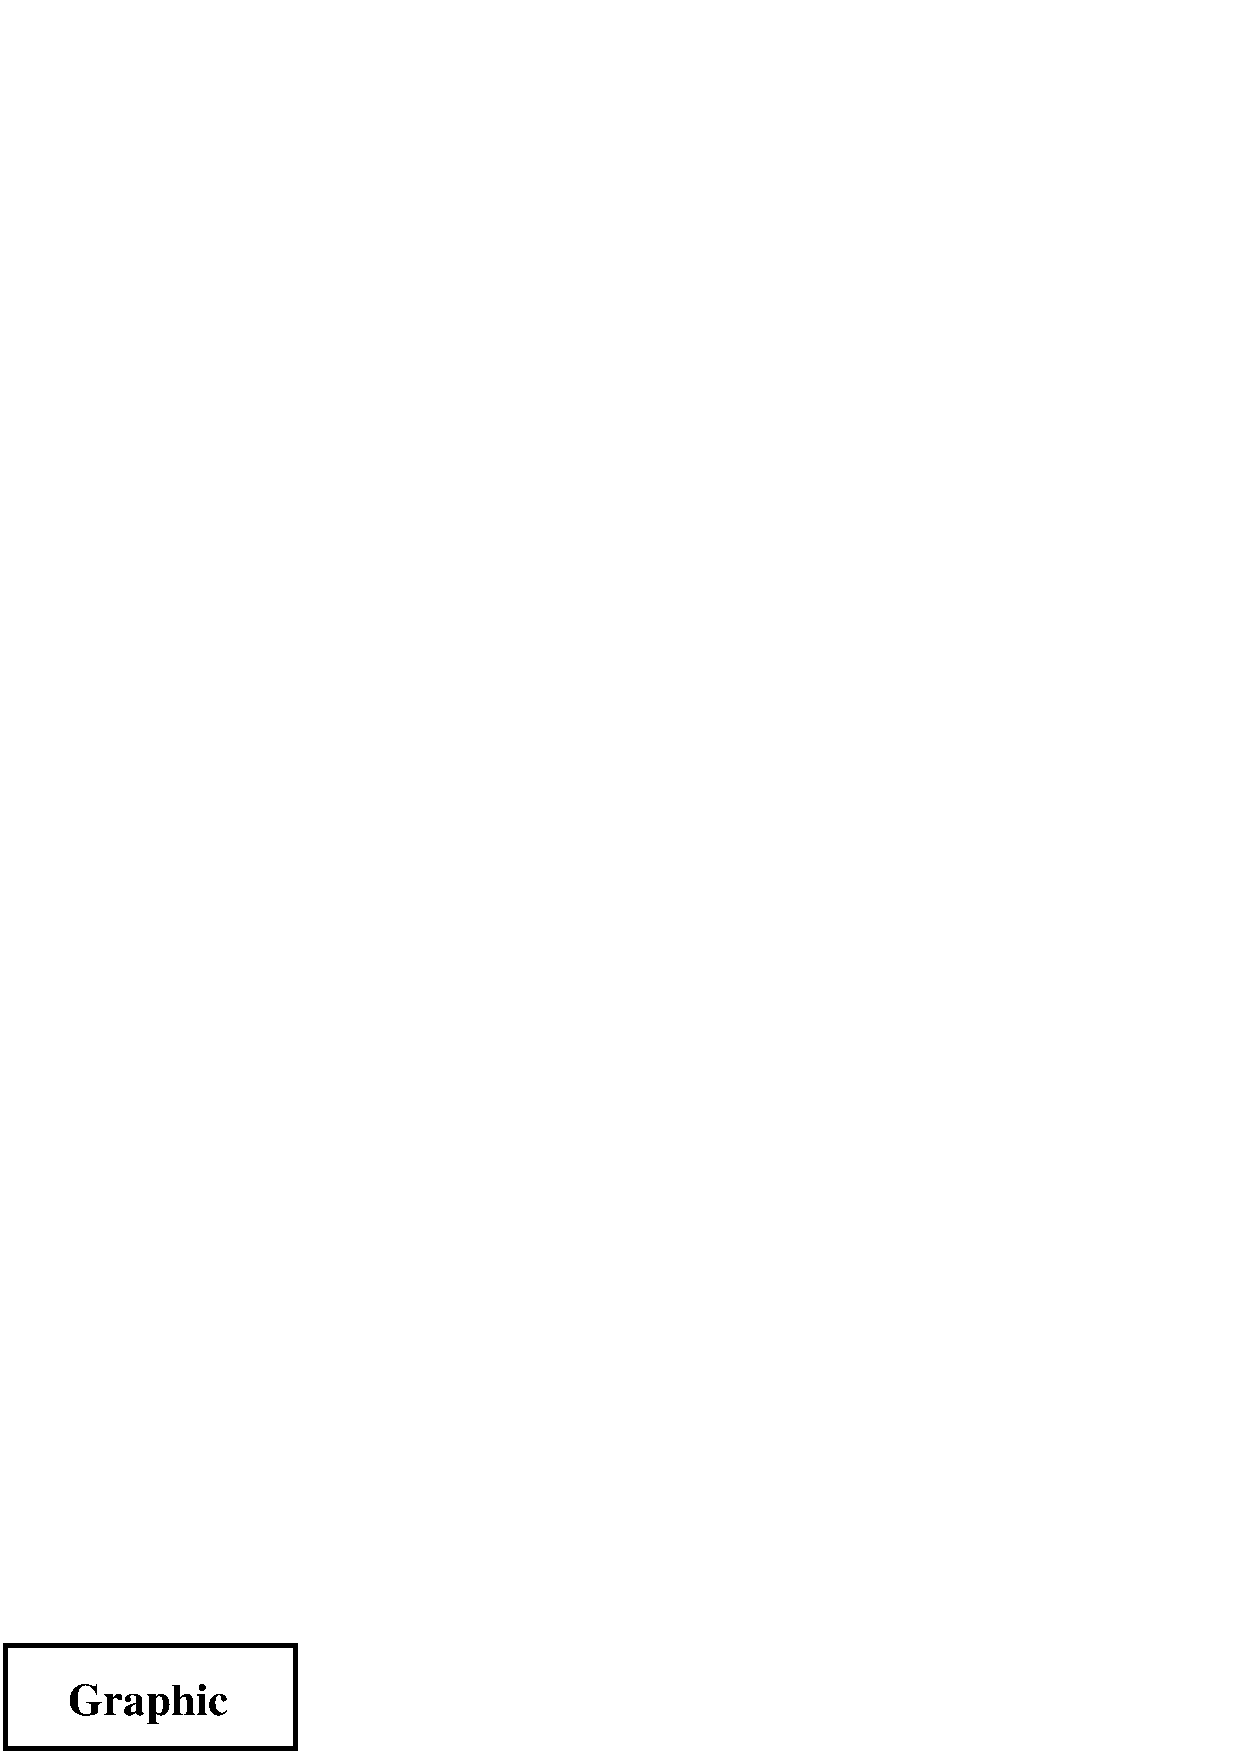
\includegraphics[width=1in,angle=-90]{graphic}
\end{center}
\end{lstlisting}
将右边的图形绕它的左下角旋转,得到如下结果:
\begin{center}
	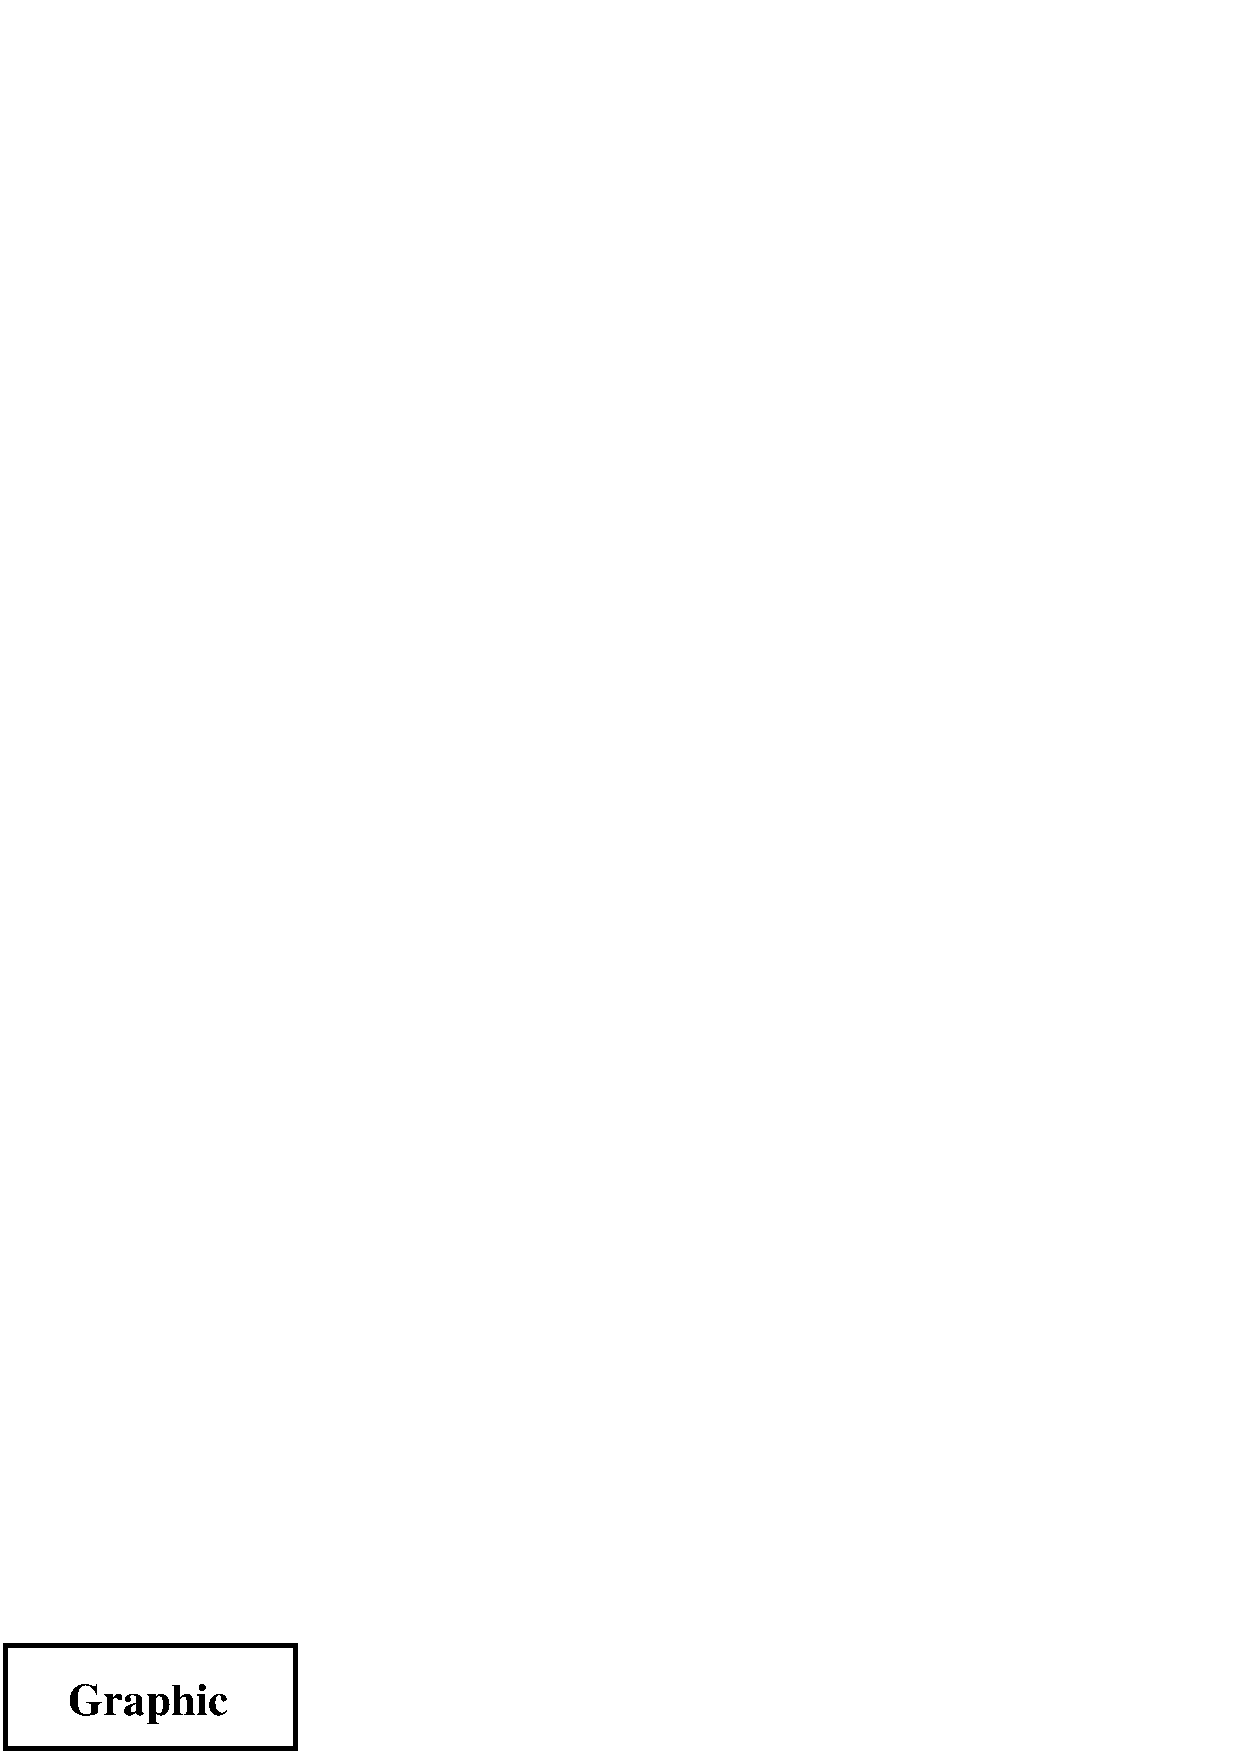
\includegraphics[width=1in]{graphic}
	\hspace{1in}
	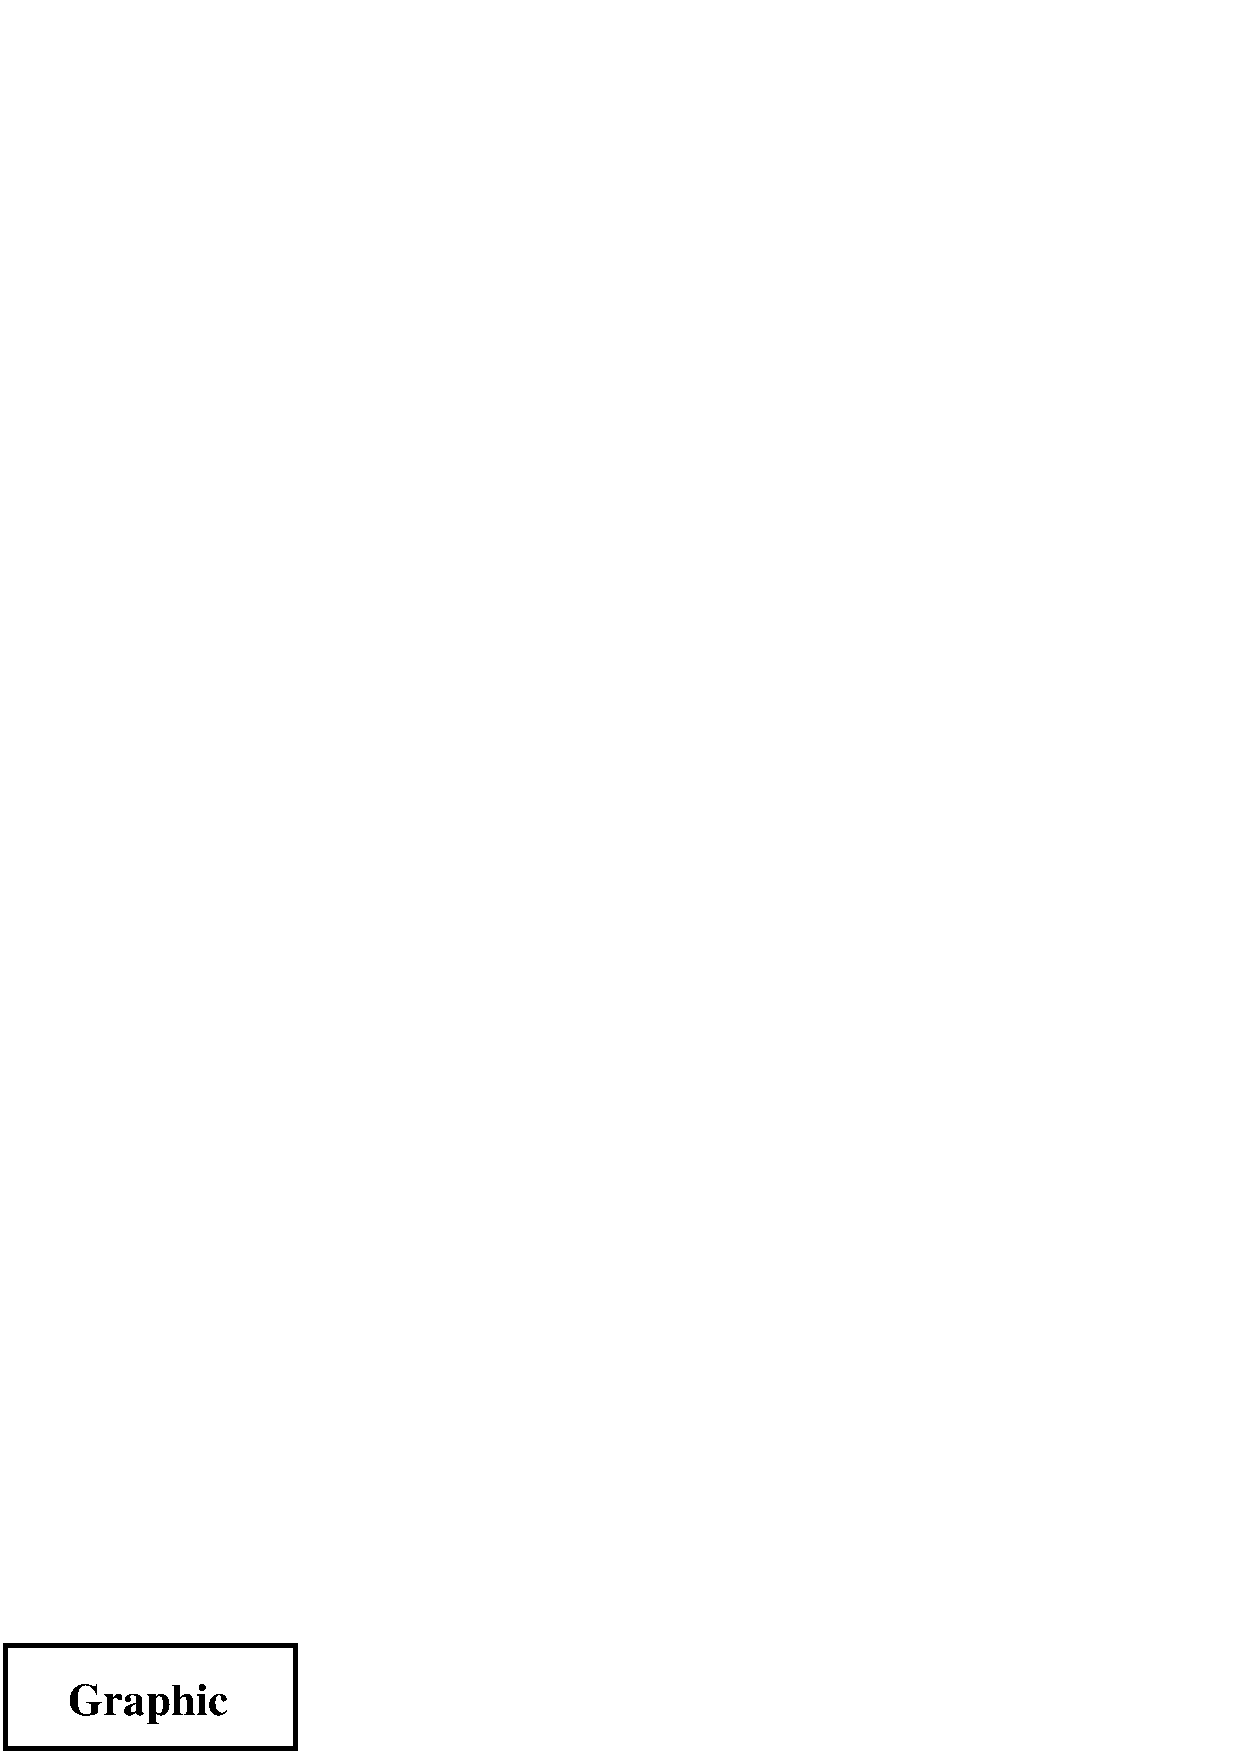
\includegraphics[width=1in,angle=-90]{graphic}
\end{center}

要想使图形的底部对齐,使用下面的命令:
\begin{lstlisting}
\begin{center}
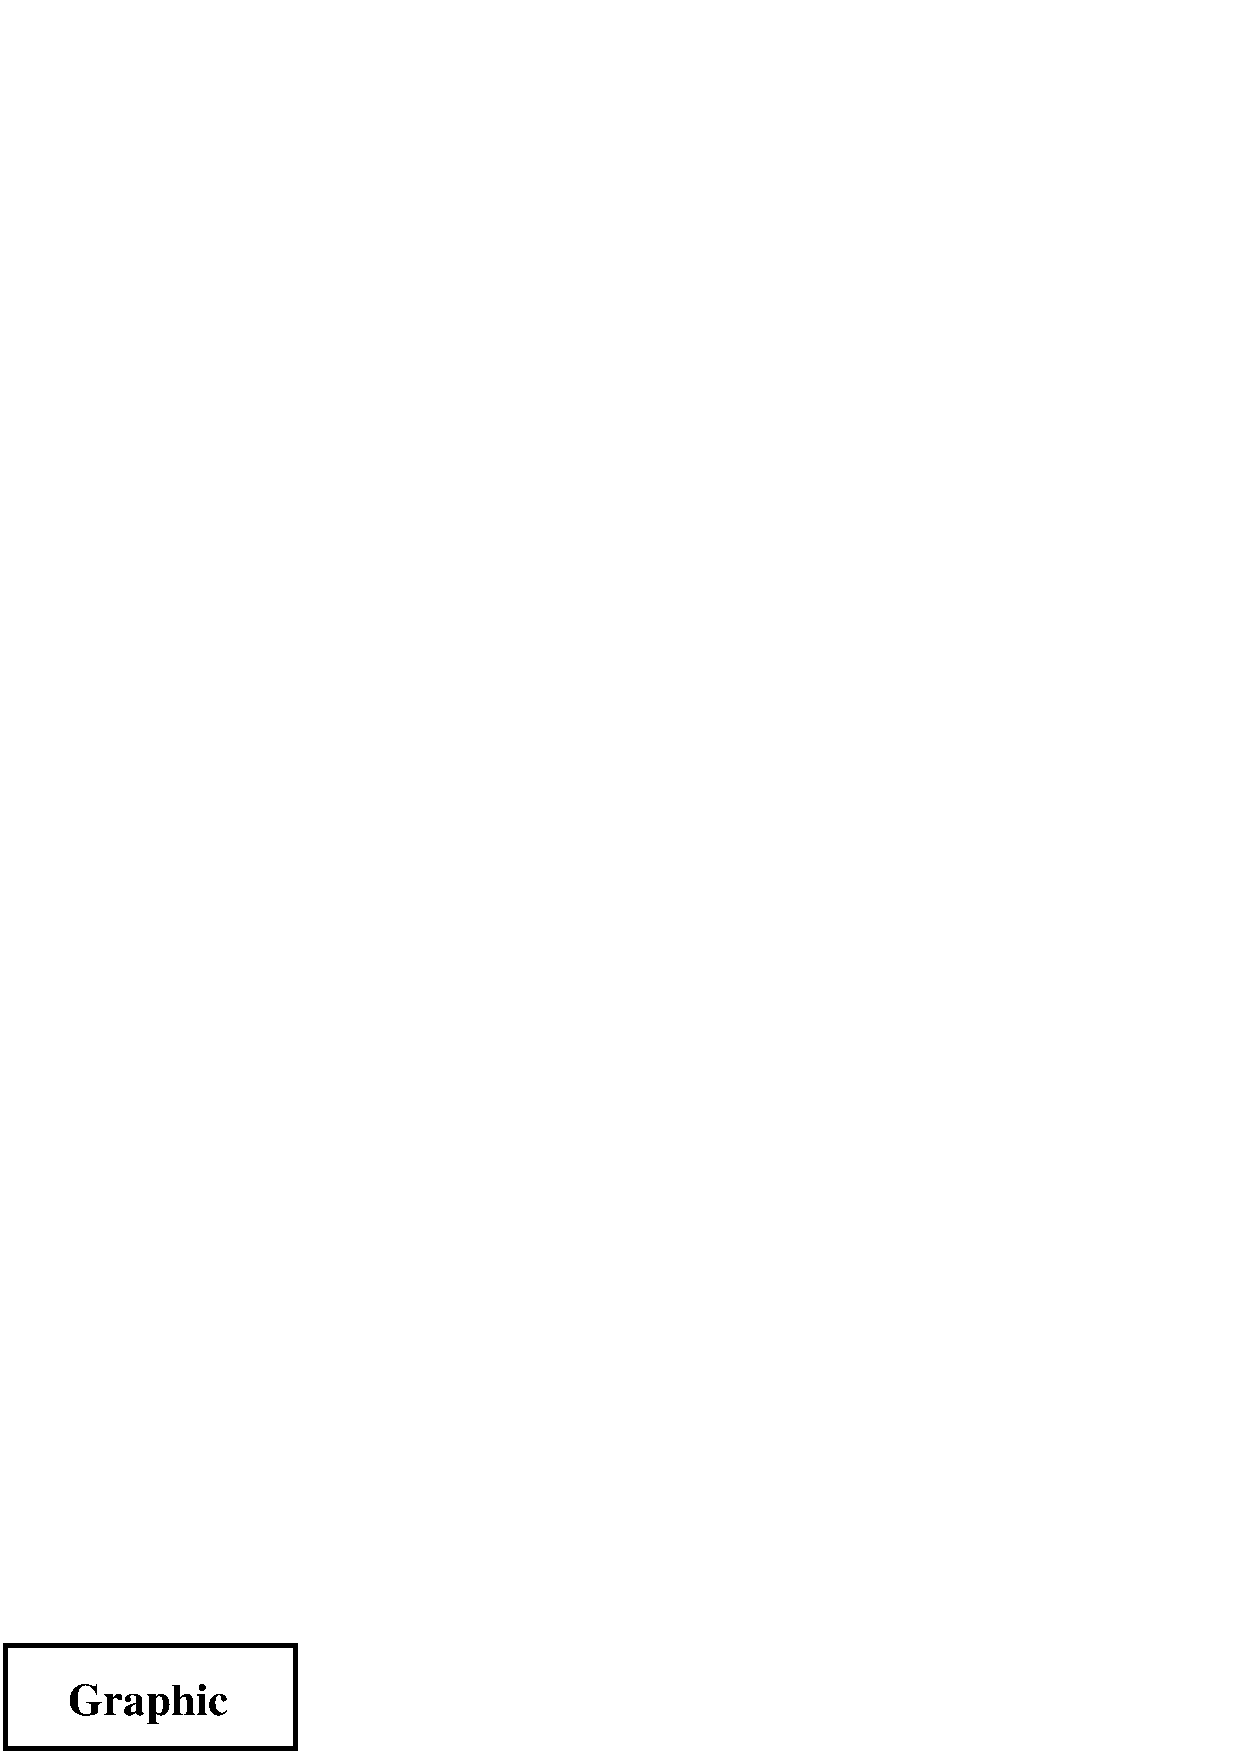
\includegraphics[width=1in]{graphic}
\hspace{1in}
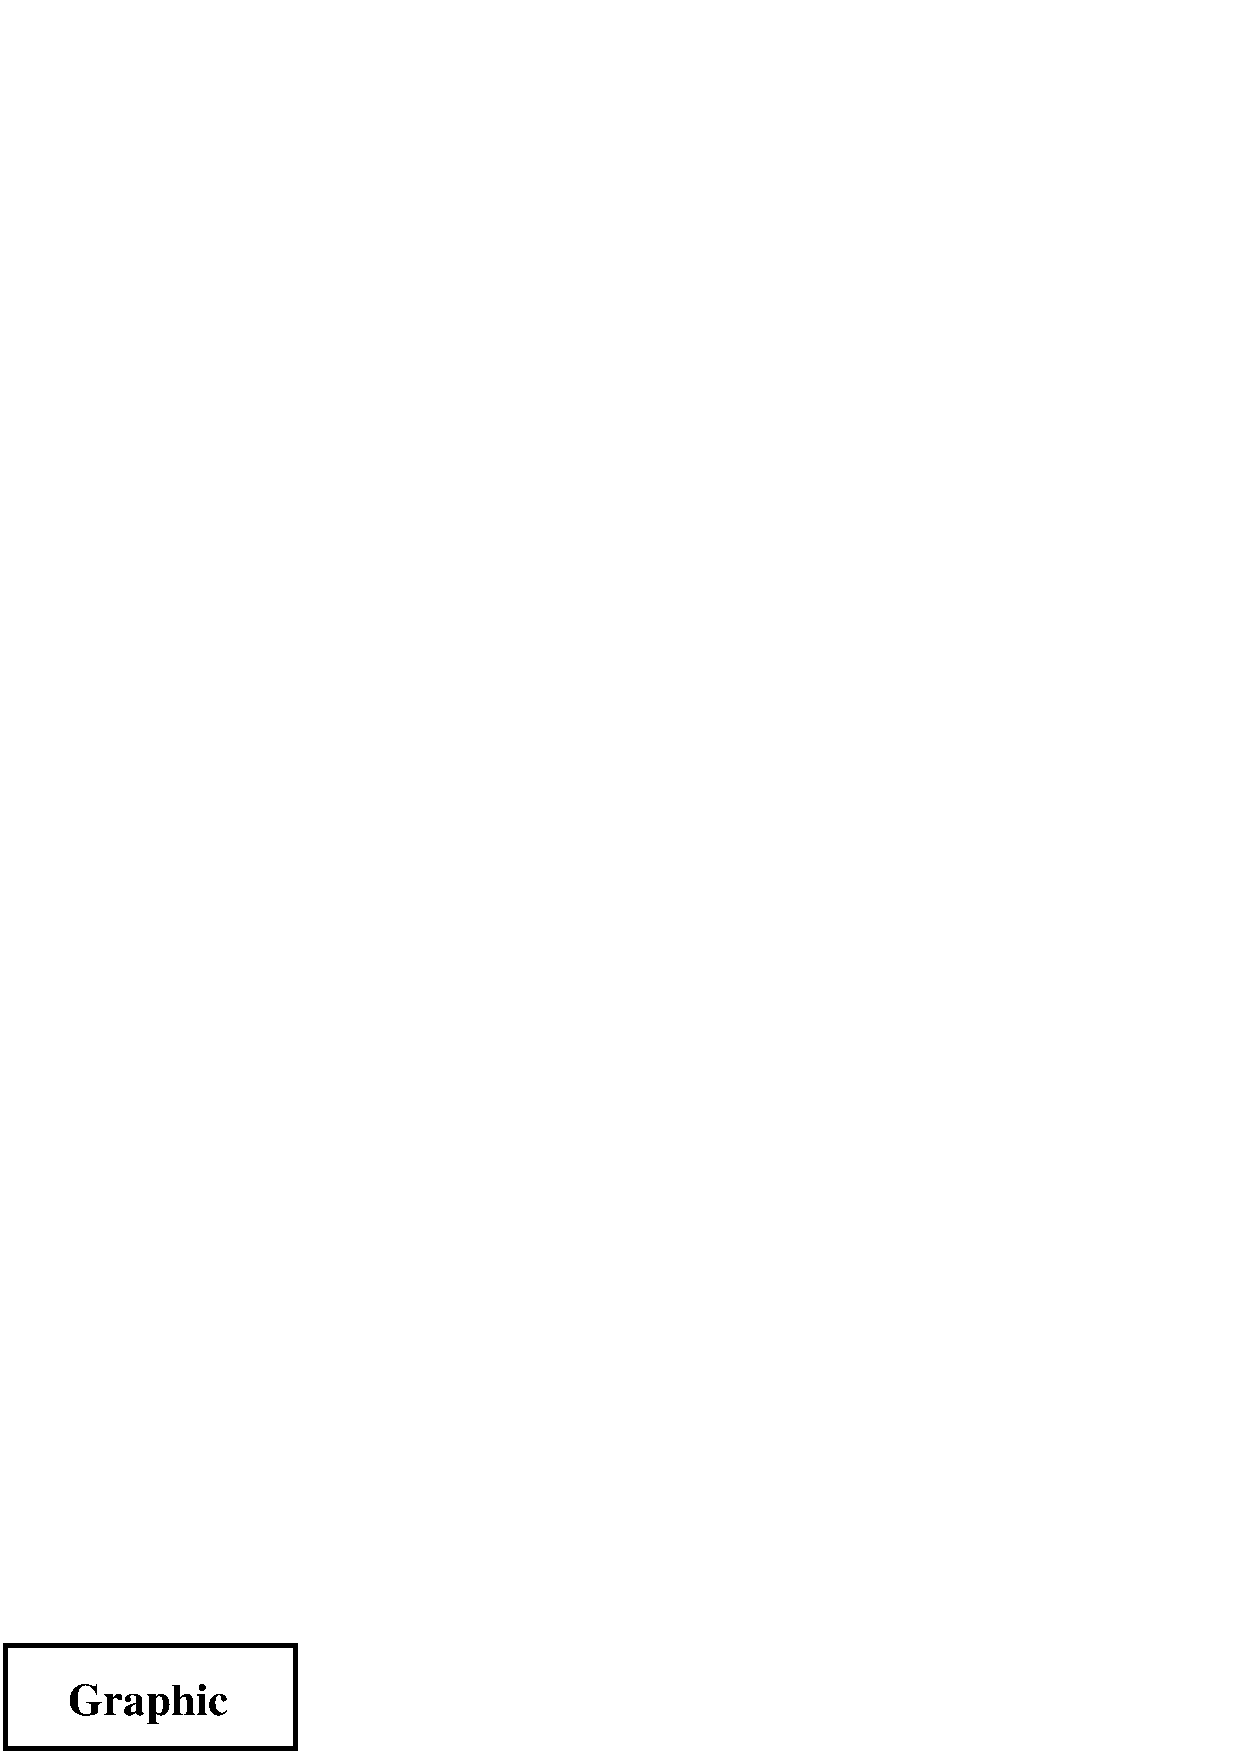
\includegraphics[width=1in,origin=br,angle=-90]{graphic}
\end{center}
\end{lstlisting}
上述命令让右边的图形绕它的右下角旋转,得到如下结果:
\begin{center}
	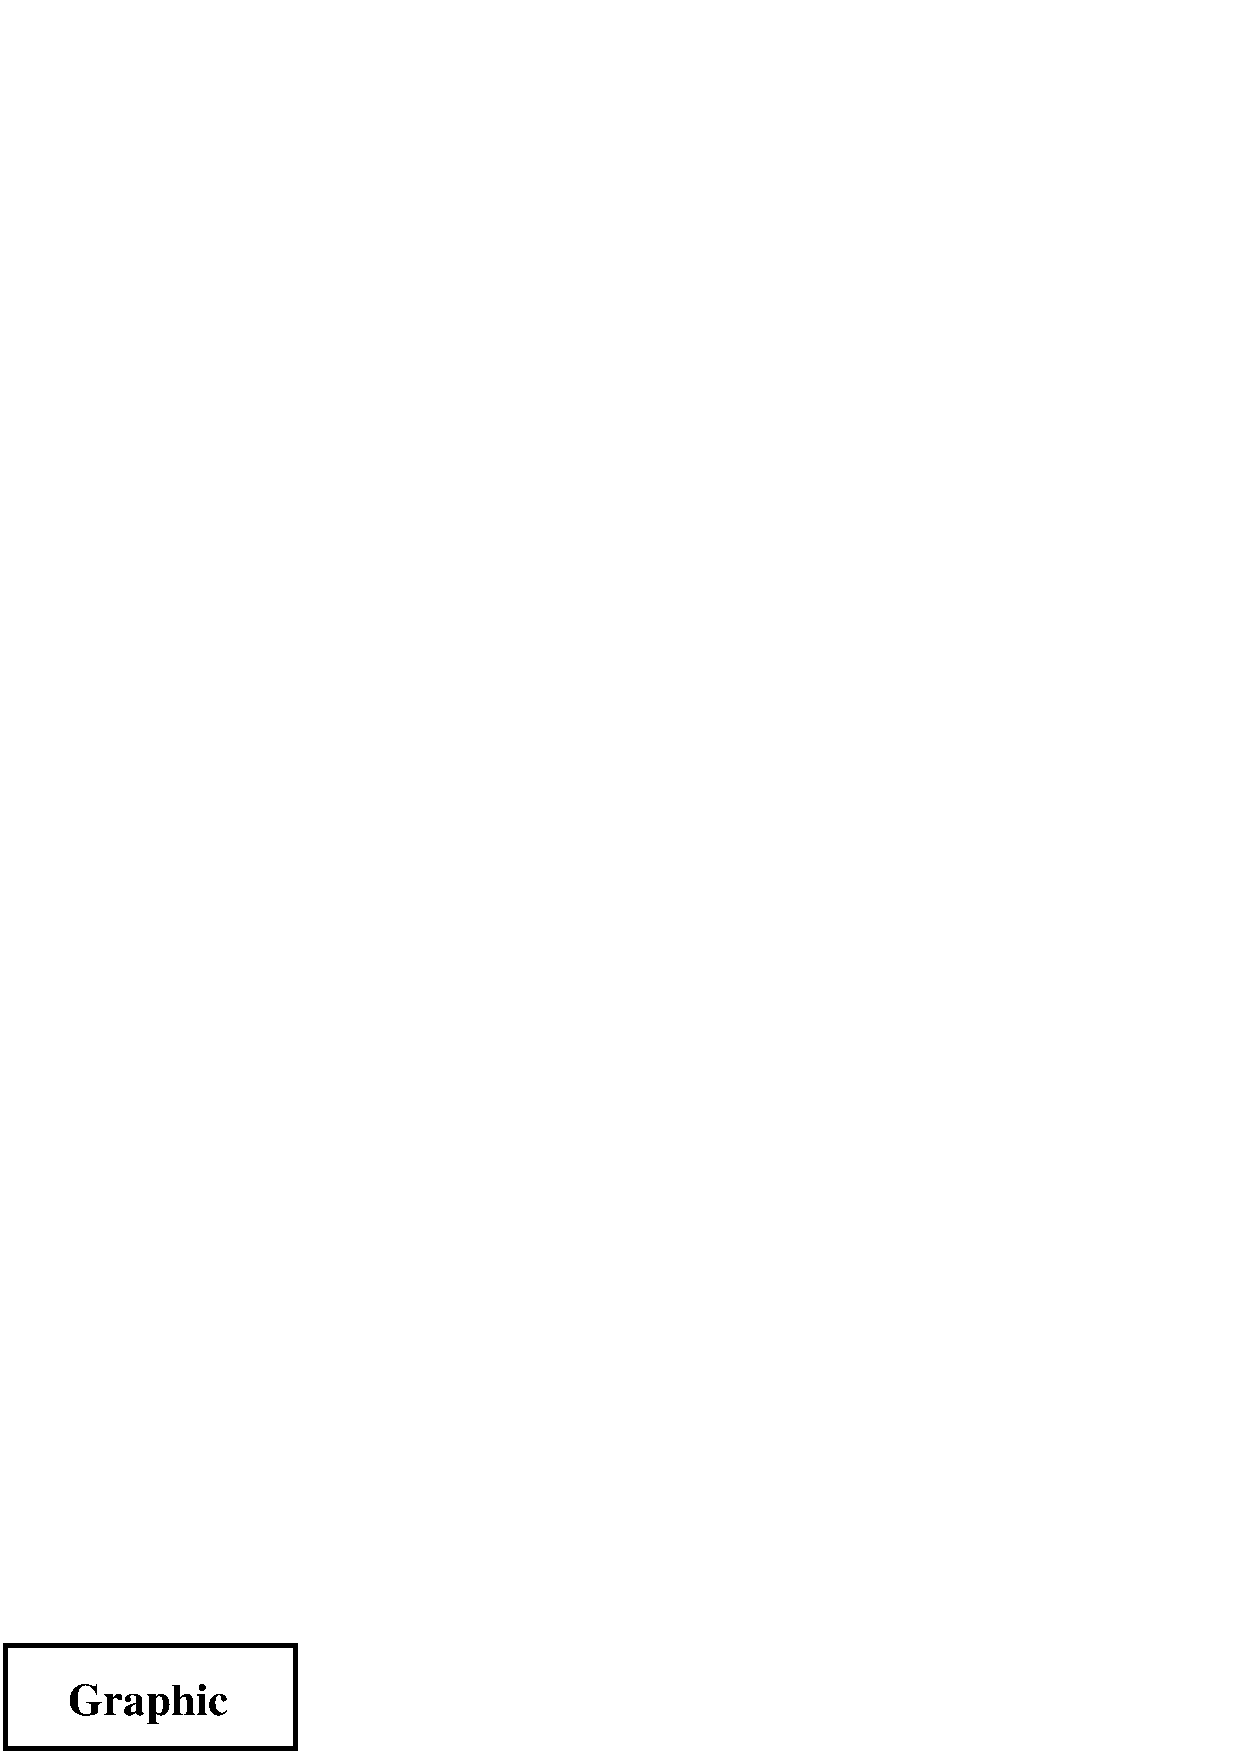
\includegraphics[width=1in]{graphic}
	\hspace{1in}
	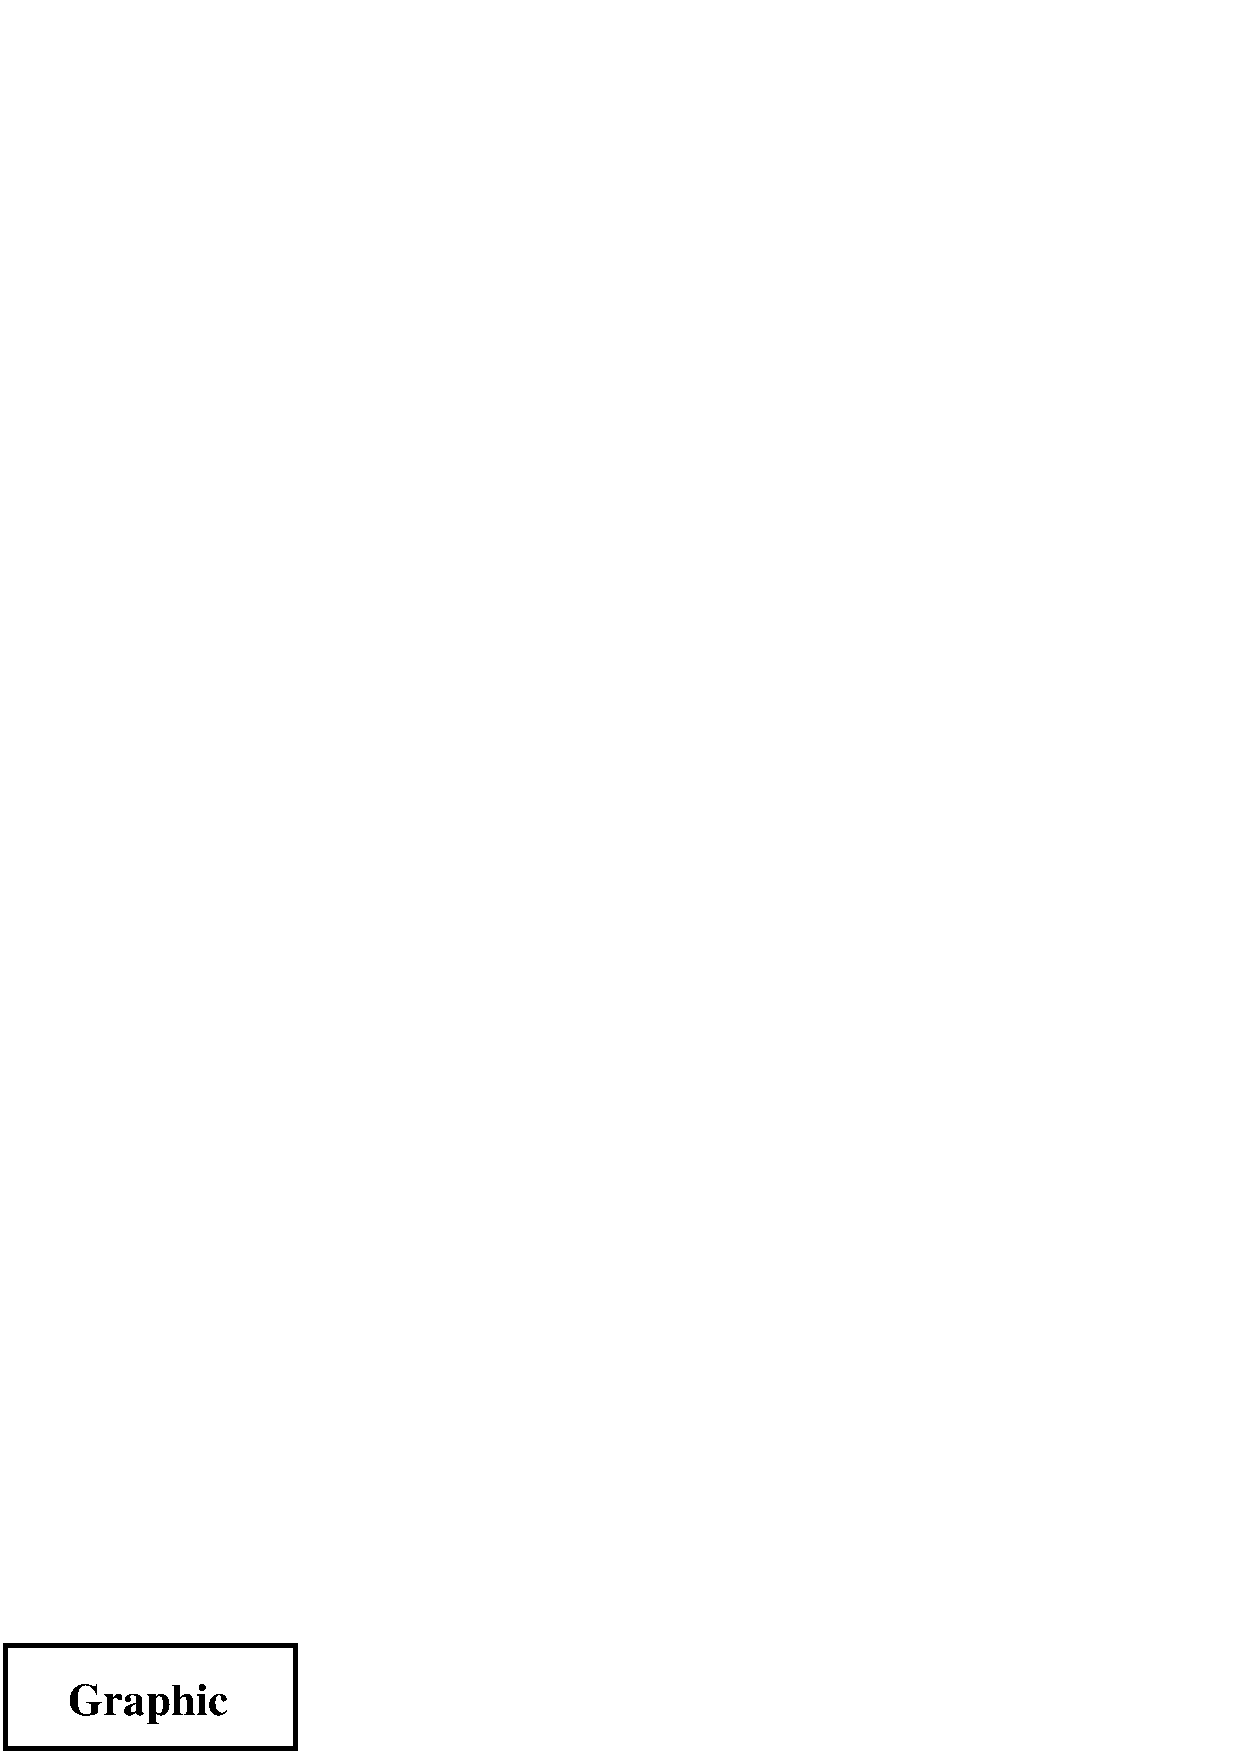
\includegraphics[width=1in,origin=br,angle=-90]{graphic}
\end{center}


\subsection{小页环境的垂直对齐}\label{ssec:minivalign}

将图形放置于 \envi{minipage} 小页环境中是经常遇到的情况下,
而且也十分实用(见第~\ref{sec:sidebyside}~节)。
当小页并列时, \LaTeX{} 会将它们的参考点垂直对齐地排列。
缺省地,小页的参考点是它的左边界的中点。
可用一个可选参数项来改变小页的参考点的位置。
\begin{description}
	\item[\opt{[b]}] 使小页的参考点与小页底行的参考点对齐。
	\item[\opt{[t]}] 使小页的参考点与小页顶行的参考点对齐。
\end{description}

注意选项 \opt{[b]} 不会将参考点置于小页的底部
(除非其底行的参考点在它的底部),
同样地,选项 \opt{[t]}~不会将参考点置于小页的顶部
(除非其顶行的参考点在它的顶部)。

当小页中只有一行时, \opt{[b]} 和 \opt{[t]} 选项得到的结果是一样的。例如:
\begin{lstlisting}
\begin{center}
\begin{minipage}[b]{.25\linewidth}
\centering
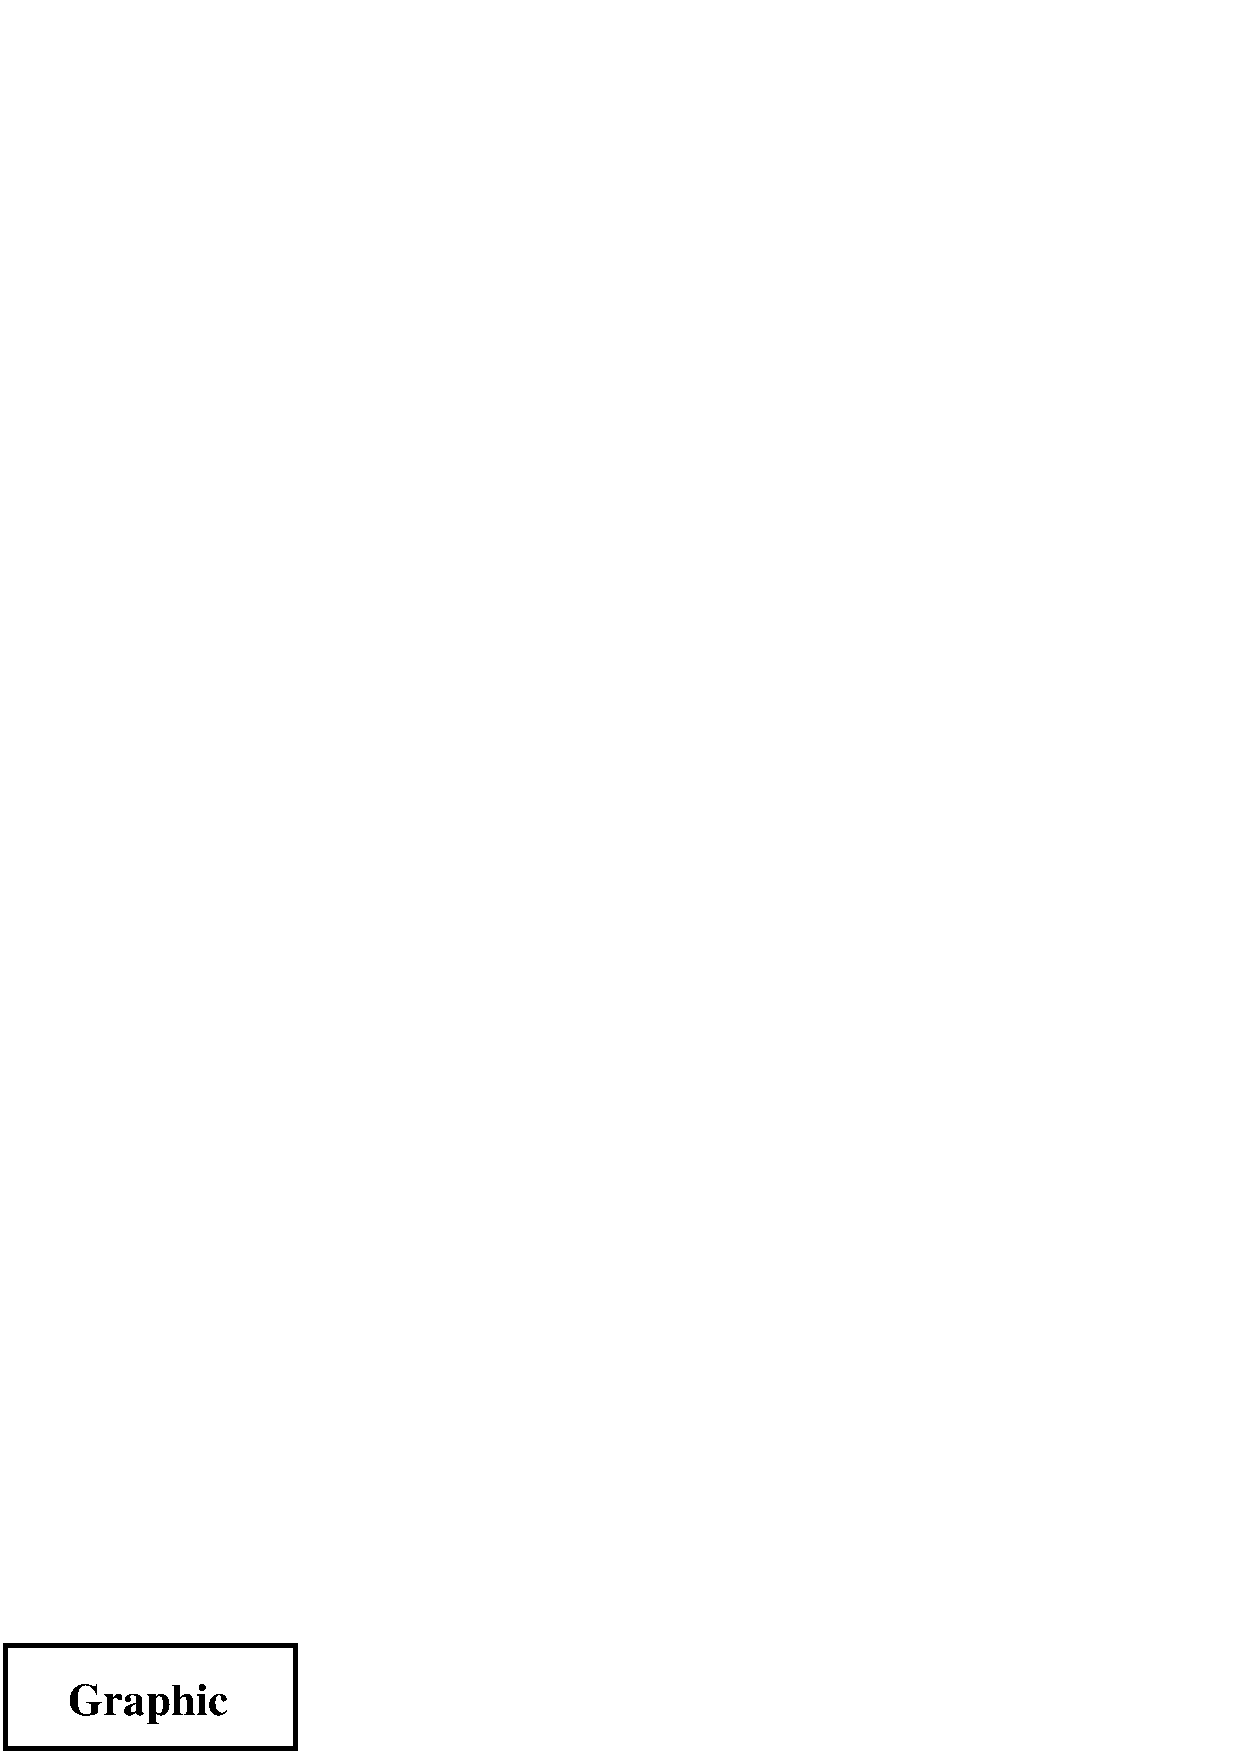
\includegraphics[width=1in]{graphic}
\end{minipage}%
\begin{minipage}[b]{.25\linewidth}
\centering
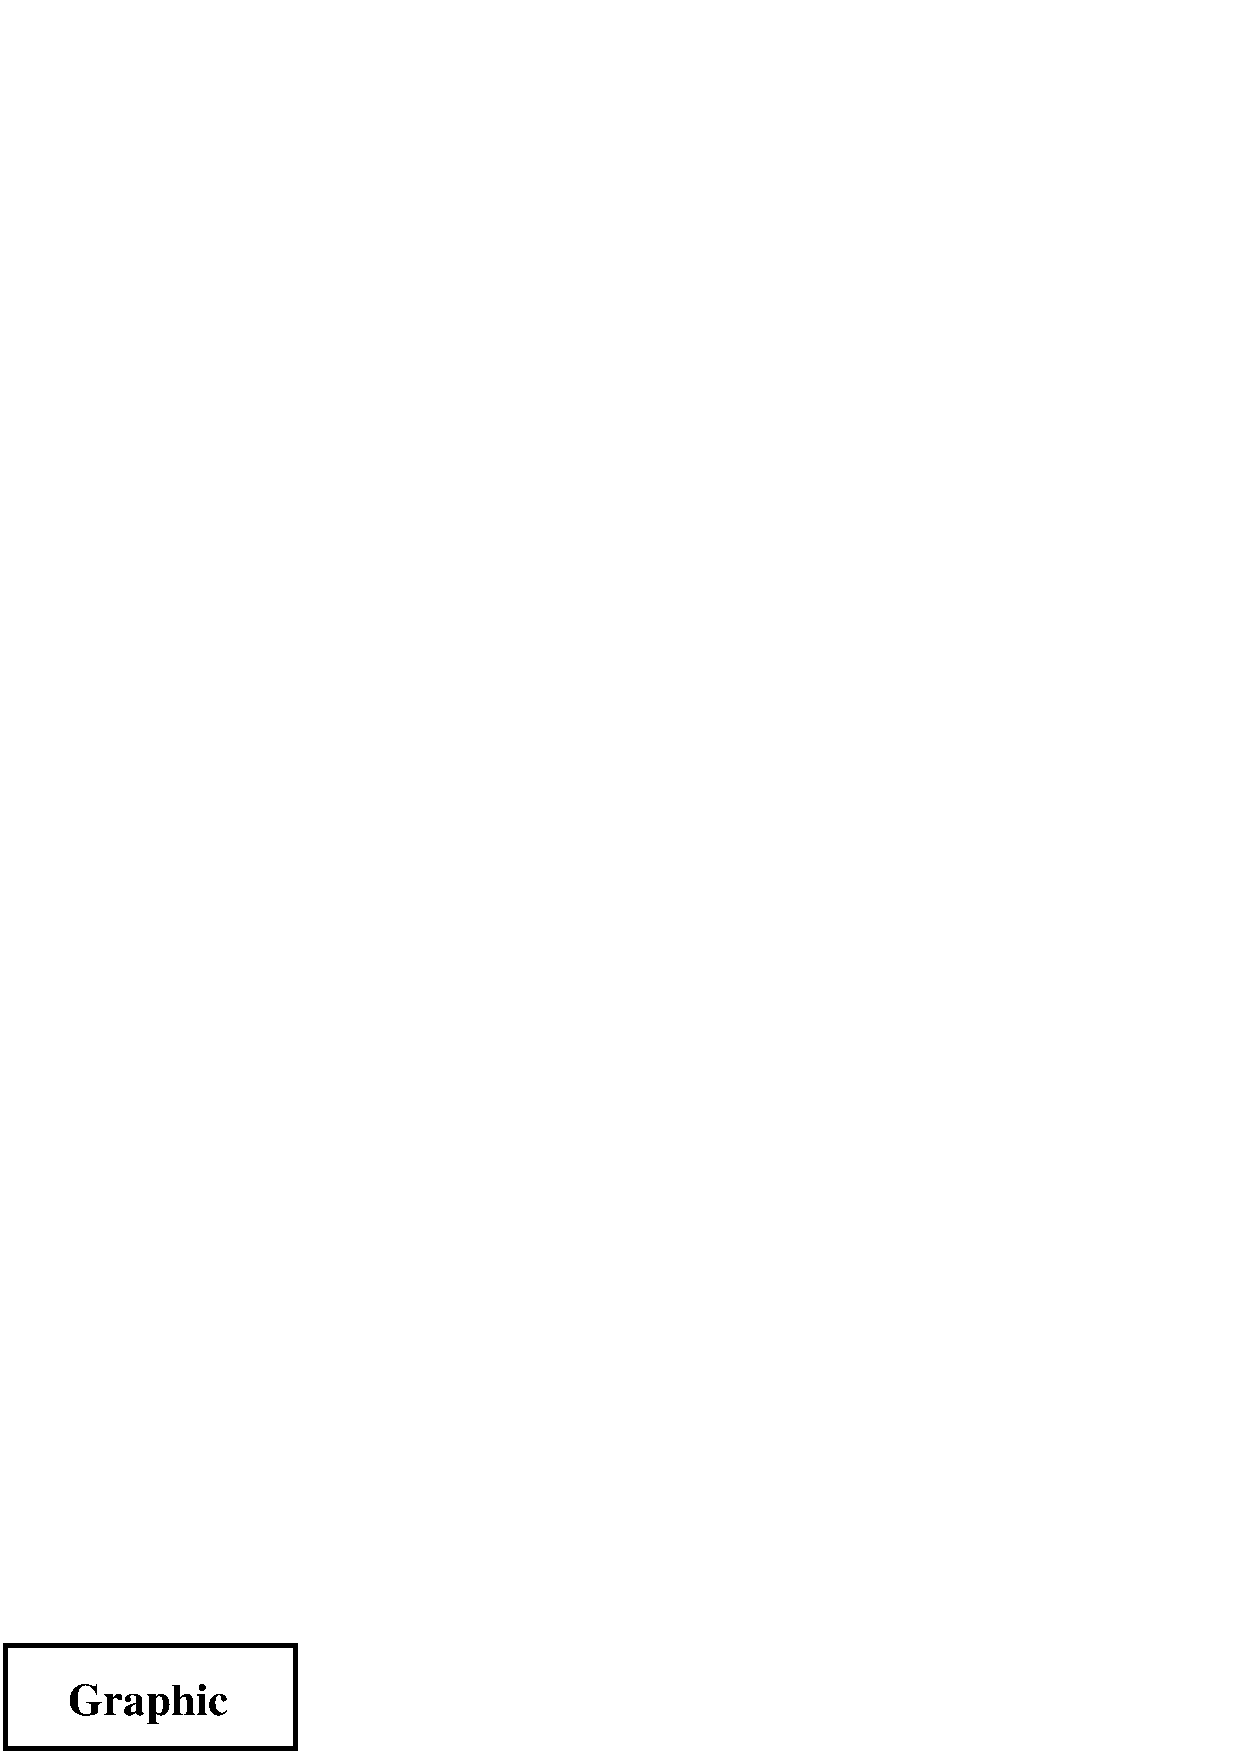
\includegraphics[width=1in,angle=-45]{graphic}
\end{minipage}
\end{center}
\end{lstlisting}
和
\begin{lstlisting}
\begin{center}
\begin{minipage}[t]{.25\linewidth}
\centering
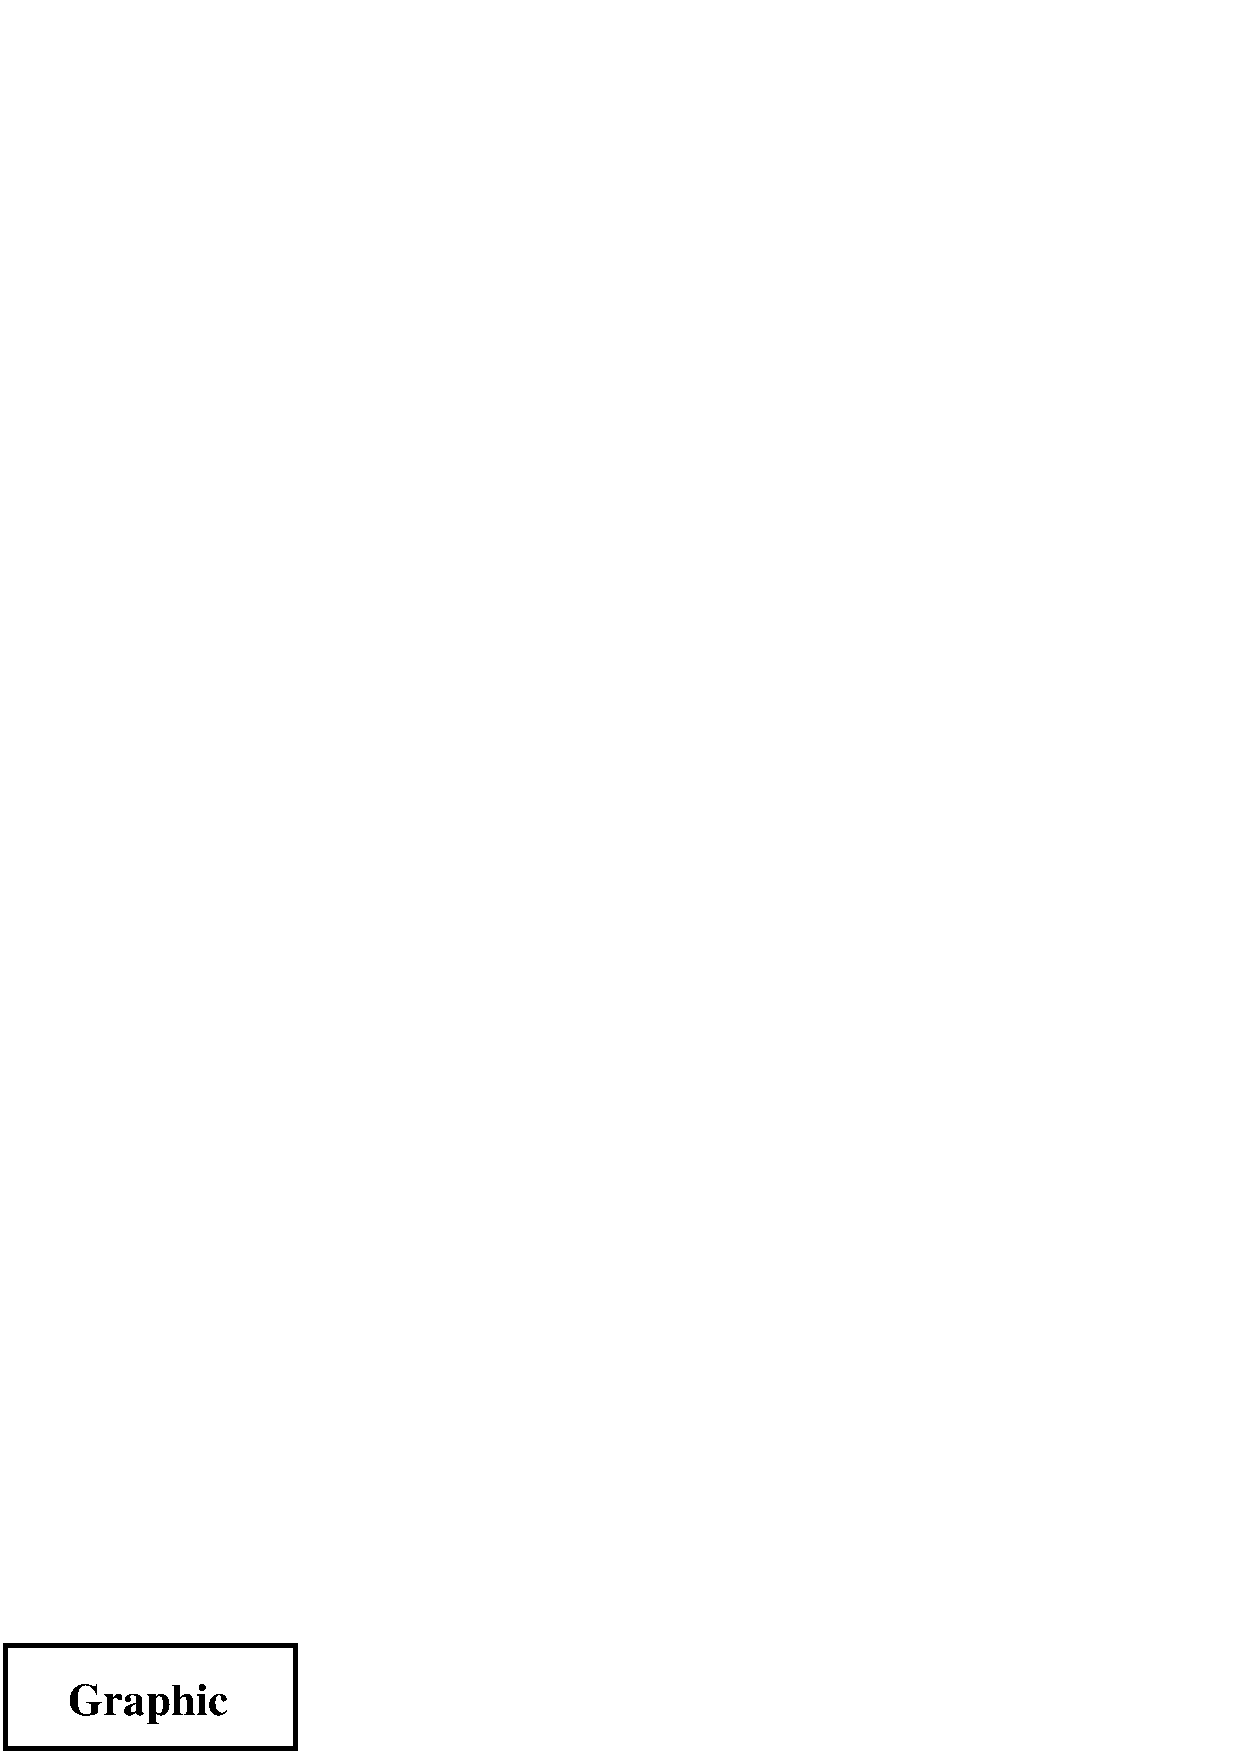
\includegraphics[width=1in]{graphic}
\end{minipage}%
\begin{minipage}[t]{.25\linewidth}
\centering
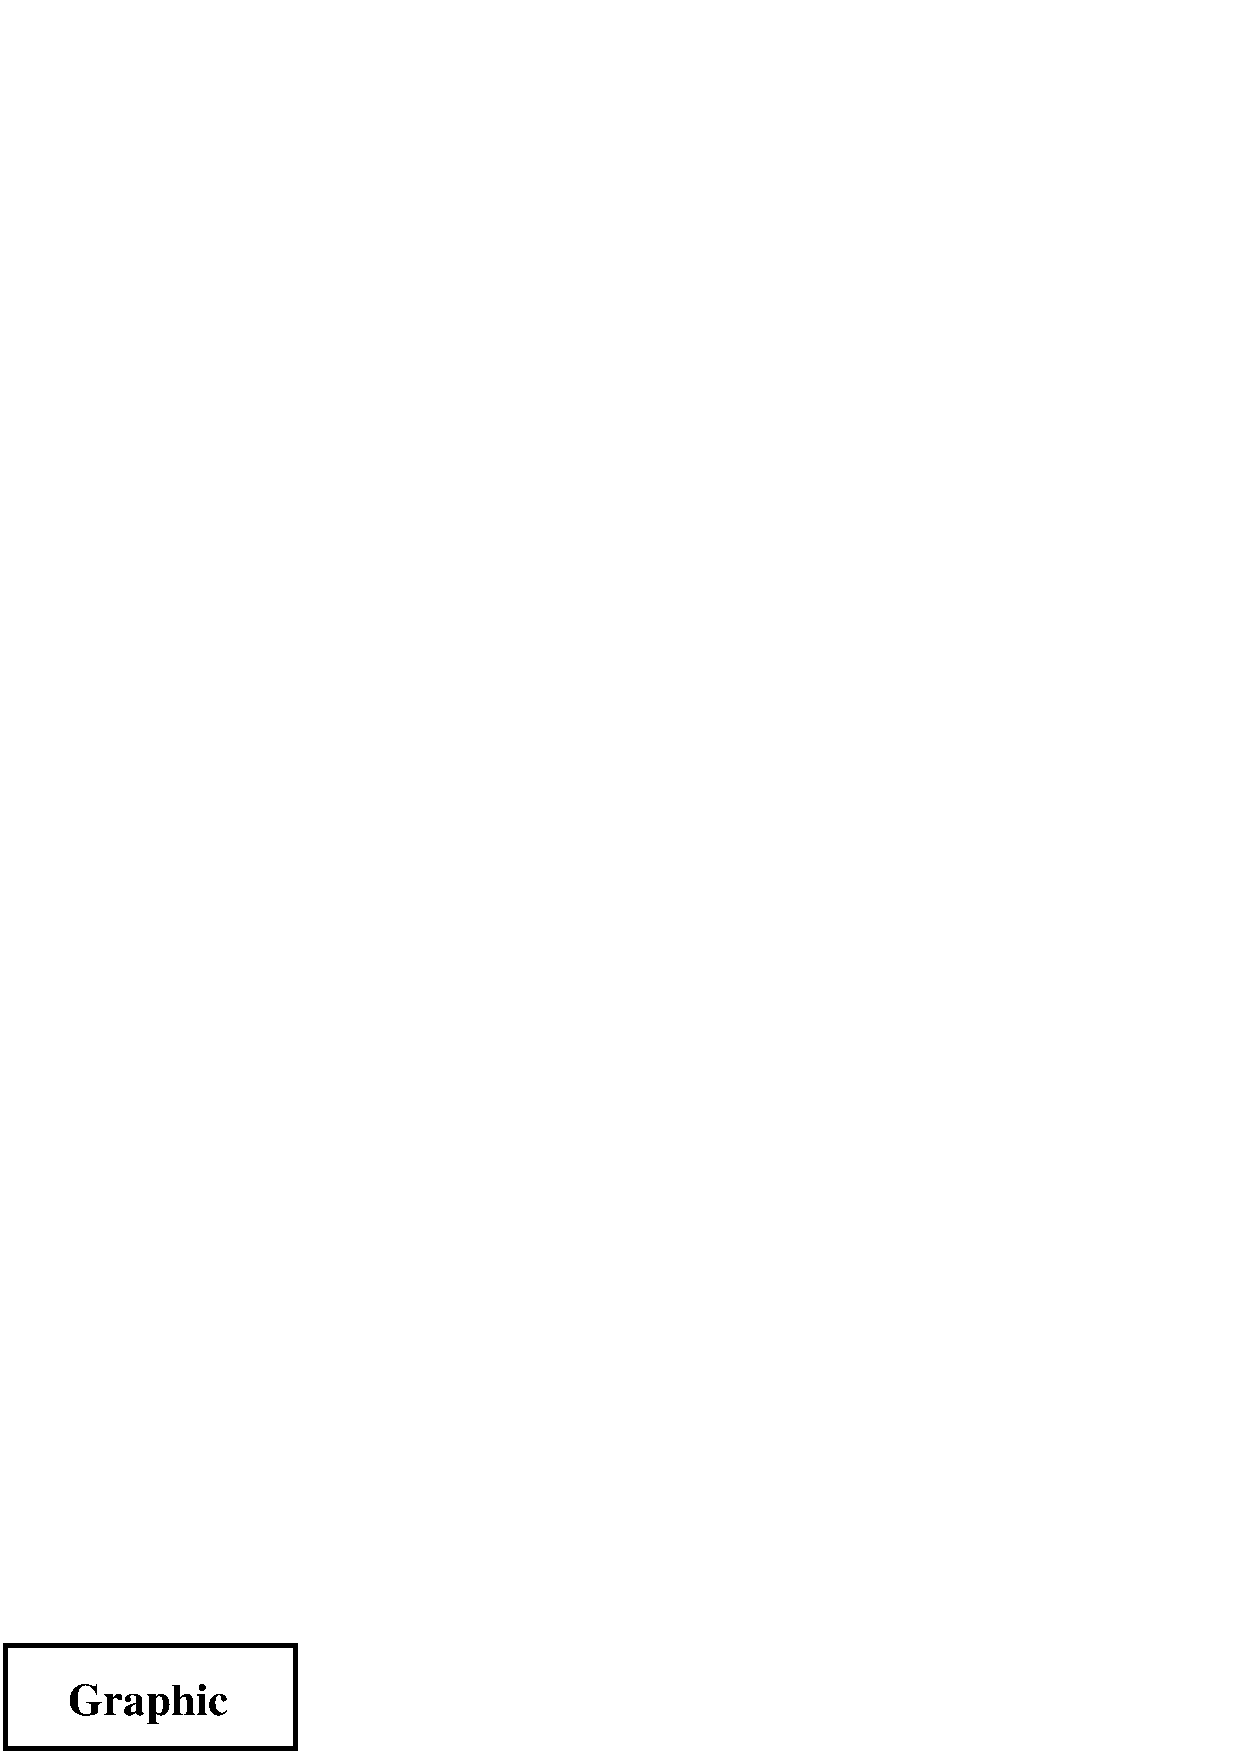
\includegraphics[width=1in,angle=-45]{graphic}
\end{minipage}
\end{center}
\end{lstlisting}
都得到图~\ref{fig:minipagesamp-1}~的结果。
在这两种情况下,小页的参考点都是图形的参考点(左下角)。
\begin{figure}
\begin{center}
	\begin{minipage}[t]{.25\linewidth}
		\centering
		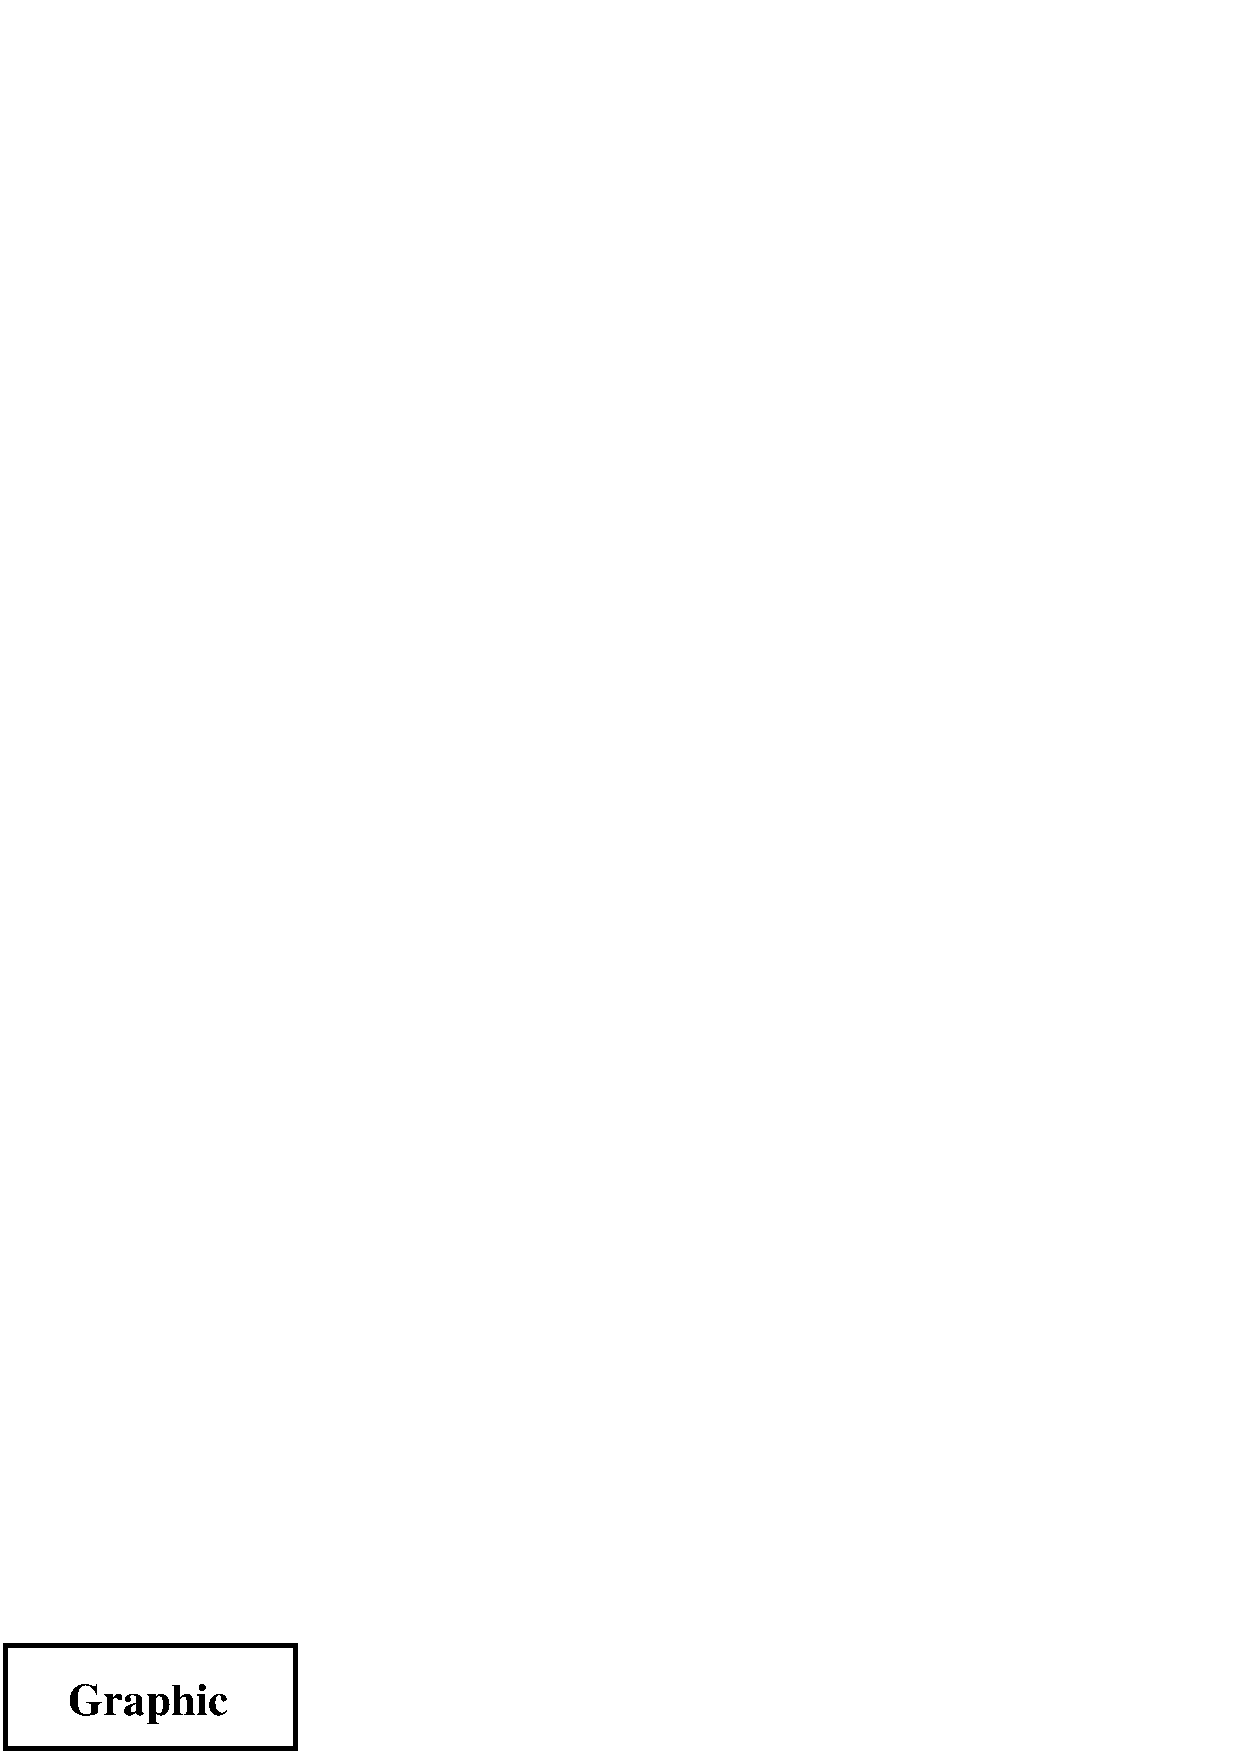
\includegraphics[width=1in]{graphic}
	\end{minipage}%
	\begin{minipage}[t]{.25\linewidth}
		\centering
		\includegraphics[width=1in,angle=-45]{graphic}
	\end{minipage}
\end{center}
\caption{带 minipage with \opt{[b]} or \opt{[t]} 选项的 \env{minipage} 环境}
\label{fig:minipagesamp-1}
\end{figure}

\subsubsection{小页的底部对齐}
让小页的底部对齐的一种方法是强制使小页的底部为其基线。
再次要注意的是,\env{minipage} 的 \opt{[b]} 选项效果是让小页最底行的基线作为小页的基线。

如果小页最底行正好是一条高和深都为零的线,
那么最后一行的参考点就是该行的底部,
这样 \opt{[b]} 选项就可使作为其基线。
类似地,如果在 \verb|\end{minipage}| 之前添加一条高度和深度为零的线,
那么 \opt{[b]} 选项就会使小页的底部作为小页的基线。
命令 \cmd{par}\cmdonearg{vspace}{0pt} 就可以产生这样高和深都为零的线段。
这时这条深度为零的线的基线就是小页的底部,
选项 \opt{[b]} 可以让小页的底部对齐了。例如:
\begin{lstlisting}
\begin{center}
\begin{minipage}[b]{.25\linewidth}
\centering
\includegraphics[width=1in]{graphic}
\par\vspace{0pt}
\end{minipage}%
\begin{minipage}[b]{.25\linewidth}
\centering
\includegraphics[width=1in,angle=-45]{graphic}
\par\vspace{0pt}
\end{minipage}
\end{center}
\end{lstlisting}
结果如图~\ref{fig:minipagesamp-2}。
\begin{figure}
\begin{center}
	\begin{minipage}[b]{.25\linewidth}
		\centering
		\includegraphics[width=1in]{graphic}
		\par\vspace{0pt}
	\end{minipage}%
	\begin{minipage}[b]{.25\linewidth}
		\centering
		\includegraphics[width=1in,angle=-45]{graphic}
		\par\vspace{0pt}
	\end{minipage}
\end{center}
\caption{底端对齐的小页环境}\label{fig:minipagesamp-2}
\end{figure}

\subsubsection{小页的顶部对齐}
当在小页的顶行加入一条高度和深度都为零的线段时,
使用 \opt{[t]} 选项使得小页的基线为它的顶部。
如果在并列的若干小页环境中都进行这样的操作,那么就可以使这些小页环境的顶端对齐。

命令 \cmdonearg{vspace}{0pt} 可以在小页的顶端插入一条高度和深度都为零的线段。
由于该条高度为零的线段的基线就位于小页的顶部,
现在使用 \opt{[t]} 选项就可以使得小页的顶部对齐了。例如:
\begin{lstlisting}
\begin{center}
\begin{minipage}[t]{.25\linewidth}
\vspace{0pt}
\centering
\includegraphics[width=1in]{graphic}
\end{minipage}%
\begin{minipage}[t]{.25\linewidth}
\vspace{0pt}
\centering
\includegraphics[width=1in,angle=-45]{graphic}
\end{minipage}
\end{center}
\end{lstlisting}
结果如图~\ref{fig:minipagesamp-3}~所示。
\begin{figure}
\begin{center}
	\begin{minipage}[t]{.25\linewidth}
		\vspace{0pt}
		\centering
		\includegraphics[width=1in]{graphic}
	\end{minipage}%
	\begin{minipage}[t]{.25\linewidth}
		\vspace{0pt}
		\centering
		\includegraphics[width=1in,angle=-45]{graphic}
	\end{minipage}
\end{center}
\caption{顶部对齐的小页环境}\label{fig:minipagesamp-3}
\end{figure}

这里小页的顶部是和当前基线对齐。
如果要求小页的顶部是和当前文本行的顶部对齐,
可用 \cmdonearg{vspace}{-\cmd{baselineskip}}。
  ~\verb+\vspace{-\baselineskip}+~来
相关专题参考~\cite[第~863--865~页]{Mittelbach2004}。


\section{两幅图像的堆叠}
本节描述如何堆叠两幅图像。
请注意这里没有检查确保顶层的图像是透明的。
如果顶层图像创建时使用非透明的背景,那么就会隐藏底层图像。

例如\footnote{
	尽管在这个例子中使用了两个 \file{eps} 图像,
	类似的代码也可以用于堆叠其它图像格式。
},
文件 \file{left.eps} 和 \file{right.eps} 包含的图像如图~\ref{fig:leftright} 所示。
使用如下命令
\begin{lstlisting}
\makebox[0pt][l]{\includegraphics{left.eps}}%
\includegraphics{right.eps}
\end{lstlisting}
就会堆叠两幅图像,如图~\ref{fig:leftrightoverlay} 所示。
堆叠两幅图像时,它们参考点(左下角)是重合的。
在这个例子中,两幅图像的自然大小是相同的,
所以不需要缩放就可以完全堆叠在一起。
其它的图像可能需要缩放
(使用 \cmd{includegraphics}、\cmd{scalebox} 或是 \cmd{resizebox} 等命令)
才能达到想要的堆叠效果。

如果没能理解 \cmd{makebox} 命令,这样的堆叠代码看起来就会显得有些不可思议。
实际上,\cmdthreeargs{makebox}{0pt}{l}{...} 命令会创建一个宽度为零的盒子。
当指定宽度时(这里是 \texttt{0 pt}),
那么排版算法就会分配这样宽度的水平空间,而不管其中内容的实际宽度是怎样。
这样,对于一个内容居左的宽度为零的盒子,
之后的\LaTeX{} 对象的排版效果就是覆盖在该盒子之上。

\begin{figure}
	\centering
	\includegraphics{left.eps}
	\caption{两幅图像的内容}\label{fig:leftright}
\end{figure}
\begin{figure}
	\centering
	\makebox[0pt][l]{\includegraphics{left.eps}}%
	\includegraphics{right.eps}
	\caption{两幅堆叠的图像}\label{fig:leftrightoverlay}
\end{figure}

\subsection{Overpic 宏包}
另一种堆叠图像的方法是使用 \pkgi{overpic} 宏包。
该宏包定义了一个图形环境,使得大小就是插图的尺寸大小。
相关细节参考 \pkg{overpic} 宏包文档~\cite{overpic-doc}。

================================================
\section{使用子目录}\label{sec:subdir}

当需要大量的图形文件时,你可能希望将它们存放到一个子目录下。例如放到
子目录~\texttt{images}~下,这时你试图用如下的命令来插入图形~\texttt{file.eps}。

\begin{Verbatim}
\includegraphics{images/file.eps}
\end{Verbatim}
仅管这种用法在大多数~Unix~和~DOS~下的~\TeX{}~里工作正常,它却有以下的问题:
\begin{description}
\item [{\CJKfamily{hei} 效率不高}]

      每当~\TeX{}~打开一个文件,该文件名就被存入~TeX{}~的内存中。
      当打开大量的文件时,因为给出子目录名增加了文件名的长度,
      这种内存的占用就容易导致~poolsize~错误(见第~\ref{sec:poolspace}~节)。
\item [{\CJKfamily{hei} 通用性差}]

      \LaTeX{}~的一大优势就是它的文件能在任何操作系统平台上使用。
      然而,在文件名中包括子目录名会使文件依赖于操作系统,如果不
      作明显的改变,上面的例子就无法在~VMS~或~Macintosh~上使用。
\end{description}

对于图形文件存于子目录下的情形,有两种办法:
\begin{enumerate}
\item 最好的方法是将子目录加到~\TeX{}~搜索路径中(见第~\ref{sec:texpath}~节)。
\item 另外一种办法是用~\ci{graphicspath}~命令来指明所用的子目录(见第
      ~\ref{sec:graphpath}~节)。不过,这比前一种方法的效率要低。
\end{enumerate}

上述两种方法都将使~\cmd{includegraphics}~自动搜索图形子目录,故可在
文件中用

\begin{Verbatim}
\includegraphics{file.eps}
\end{Verbatim}
来替代

\begin{Verbatim}
\includegraphics{images/file.eps}
\end{Verbatim}

\subsection{\TeX{}~搜索路径}\label{ssec:texpath}

因为不同的~TeX~软件设置搜索路径的方法不完全一样,所以很难提供一个
普遍适用的范例。本节所用的例子是基于~Unix~下的~web2c/te\TeX{}~的。
其它版本的~\TeX{}~也大致采用相似的策略。

对~Unix~下的~web2c/te\TeX{}~而言,改变~TeX~的搜索路径可通过设
置环境变量~\texttt{TEXINPUTS}~来实现。如使用~\texttt{csh},
\begin{Verbatim}[xleftmargin=1cm]
setenv TEXINPUTS /dir1:/dir2:
\end{Verbatim}
会使~\TeX{}~在搜索缺省的目录前先搜索~\texttt{/dir1}~和~\texttt{/dir2}。
如果省掉最后的~\texttt{:},那么在搜索完~\texttt{/dir1}~和~\texttt{/dir2}
~后~\TeX{}~将不再搜索缺省的目录。如设
\begin{Verbatim}[xleftmargin=1cm]
setenv TEXINPUTS :/dir1:/dir2
\end{Verbatim}
则使~\TeX{}~在搜索缺省的目录后再搜索~\texttt{/dir1}~和~\texttt{/dir2}。
而
\begin{Verbatim}[xleftmargin=1cm]
setenv TEXINPUTS /dir1::/dir2
\end{Verbatim}
则使~\TeX{}~在搜索~\texttt{/dir1}~后接下来搜索缺省的目录,最后再
搜索\texttt{/dir2}。

在一个目录后面加上~\texttt{//}~使得此目录下的所有子目录都将被搜索。
例如:
\begin{Verbatim}[xleftmargin=1cm]
setenv TEXINPUTS /dir1//:/dir2:
\end{Verbatim}
会使~\TeX{}~搜索~\texttt{/dir1}~的所有子目录。使用~\texttt{//}~要
小心,如果一目录下的文件和子目录特别多的话,它会使~\TeX{}~的搜索速度
变得很慢。

若使用~\texttt{sh},可用命令
\begin{Verbatim}[xleftmargin=1cm]
TEXINPUTS="/dir1:/dir2:"; export TEXINPUTS
\end{Verbatim}
来设置环境变量~\texttt{TEXINPUTS}。

当~\LaTeX~在~\TeX{}~搜索路径中找到文件时,并不将目录名也写到~DVI~文件中,
因此,旧版本的~\texttt{dvips}~和~\texttt{xdvi}~由于不会
搜索~\TeX{}~的搜索路径,可能会找不到该文件(见第~\ref{sec:dvips}~节)。

\subsection{图形文件搜索路径}\label{ssec:graphpath}

缺省地,~\LaTeX{}~在~\TeX{}搜索路径中寻找图形文件。除此之外,~\LaTeX{}~还
会搜索由~\ci{graphicspath}~给出的目录。例如:
\begin{Verbatim}[xleftmargin=1cm]
\graphicspath{{dir1/}{dir2/}}
\end{Verbatim}
告诉~\LaTeX{}~也从目录~\texttt{dir1/}~和~\texttt{dir2/}~下寻找图形文件。
对~Macintosh~来说,上面的命令改为:
\begin{Verbatim}[xleftmargin=1cm]
\graphicspath{{dir1:}{dir2:}}
\end{Verbatim}

很重要的一点是,搜索由~\cmd{graphicspath}~给出的目录要比由
~\texttt{TEXINPUTS}~给出的目录慢的多。更进一步说,搜索由~\cmd{graphicspath}~
给出的目录要占用一定的~pool space~(见第~\ref{sec:poolspace}节)。
鉴于~\cmd{graphicspath}效率不高,所以不推奖使用这一命令,
最好的办法就是将要使用的目录加到~\TeX{}~搜索路径中去(见
第~\ref{sec:texpath}~节)。

\subsection{节约~~Pool~~空间}\label{ssec:poolspace}

\TeX{}为其内部的字符串的传递保留了一部分内存空间,称为~\textit{pool space}
\index{pool space@\textsl}。每当~\TeX{}~打开一文件或试图打开一文件,
就会有一部分~pool space~被永久性分配。当打开一个很大的文件时,这种内存的
丢失会导致~\TeX~耗光它的~pool size,产生如下的错误讯息:
\begin{Verbatim}[xleftmargin=1cm]
! TeX capacity exceeded, sorry [poolsize=72288]
\end{Verbatim}
因为已分配的~pool space~是文件名长度的函数,所以若其中带有子目录名会
使~pool space~问题更加恶化。

除了最新版的基于~web2c~的~\TeX{}~软件和一些商业软件外,增加~poolsize~的
唯一办法就是重新编译~\TeX{}。所幸的是,通常用下面这些节约~pool space~的
办法就可以解决问题。

\begin{itemize}
\item 避免用过长的文件名。
\item 不要把子目录名包括进来
      \begin{Verbatim}
      \includegraphics{images/file.eps}
      \end{Verbatim}
      取而代之的是将子目录加到~\TeX{}~搜索路径中或不要把图形文件放在
      子目录下。
\item 不要使用~\cmd{graphicspath}~命令。
      \begin{Verbatim}
      \graphicspath{{dir1/}{dir2/}}
      ...
      \includegraphics{file.eps}
      \end{Verbatim}
      将使~\cmd{includegraphics}~命令试图打开下列文件:
      \begin{Verbatim}[xleftmargin=1.5cm]
      file.eps
      dir1/file.eps
      dir2/file.eps
      \end{Verbatim}
      这每一次打开文件的尝试都会消耗~pool space。应该用更改~\TeX{}~搜索路径
      的办法来替代使用命令~\cmd{graphicspath}。
\item 给出全部的文件名,不要省略文件的扩展名(特别地,像~.eps)。在缺省的
      ~\cmd{DeclareGraphicsExtensions}~定义下,命令
      \begin{Verbatim}
      \includegraphics{file}
      \end{Verbatim}
      将使~\cmd{includegraphics}~命令试图打开下列文件:
      \begin{Verbatim}[xleftmargin=1.5cm]
      file.eps
      file.ps
      file.eps.gz
      file.ps.gz
      file.eps.Z
      \end{Verbatim}
     若是再加上使用~\cmd{graphicspath},会导致效率极低。

     最好将~\cmd{DeclareGraphicsExtensions}~中定义的扩展名集减到最小,
     这样在使用省略扩展名的文件时会好些。
\end{itemize}

\section{压缩图形文件和非~~EPS~~文件的使用}\label{sec:noneps}

当使用~\texttt{dvips}~时,使用者可定义一个命令来在插入图形文件之前对它进行操作。
这样,如果设定此命令为一解压缩命令,就可以使用压缩的图形文件。如果设定此命令为
一图形格式转换命令,就可以使用非~EPS~图形文件。考虑到目前为止~DVI~到~PS~的
转换程序中只有~\texttt{dvips}~具有这种功能,本节所介绍的内容都需要
~\texttt{dvips}~的支持。使用者需要在使用~\textsf{graphicx}~宏包时
设定使用~\texttt{dvips}~选项。这可以通过在~\cmd{documentclass}~命令
中进行全局设定:

\begin{Verbatim}[xleftmargin=1cm]
\documentclass[dvips,11pt]{article}
\end{Verbatim}
或者在~\cmd{usepackage}~中设定~\textsf{graphicx}~的使用~\texttt{dvips}~选项为:

\begin{Verbatim}[xleftmargin=1cm]
\usepackage[dvips]{graphicx}
\end{Verbatim}
推荐使用第一种方法,因为它将~\texttt{dvips}~这一选项传递给所有的宏包。

当使用一个支持管道\realfootnote{例如,~Unix~支持管道而~DOS~则不支持}的操作系统
时,~\cmd{DeclareGraphicsRule}~命令(见第~\ref{sec:derule}~节)定义一个
对文件进行操作的命令。若为解压缩命令,则可允许使用压缩的图形文件。
若为图形格式转换命令,则可允许使用非~EPS~图形文件。当使用不支持管道的操作系统
时,这种即时转换的命令是不允许的,这时只好将所有的图形文件都存为非压缩
的~EPS~格式。

\clearpage

\subsection{压缩 EPS 文件的例子}\label{ssec:compresseps}

使用压缩~EPS~文件的步骤是:
\begin{enumerate}
\item 创见一个~EPS~文件(比如说~\texttt{file.eps})。
\item 将它的~BoundingBox~存放到另外一文件中(~\texttt{file.eps.bb})。
\item 压缩~EPS~文件,比如用~Unix~命令:
      \begin{Verbatim}[xleftmargin=1cm]
      gzip -9 file.eps
      \end{Verbatim}
      得到压缩文件~\texttt{file.eps.gz}。这里~\texttt{-9}(或者~\texttt{-best})
      选项表示最佳压缩。
\item 在~\cmd{includegraphics}前声明适当的
      ~\cmd{DeclareGraphicsRule}~命令。使得~\LaTeX{}~知道如何
      处理特殊后缀的文件(见第~\ref{sec:derule}~节)。例如:
      \begin{Verbatim}
      \documentclass[dvips]{article}
      \usepackage{graphicx}
      \begin{document}
      \DeclareGraphicsRule{.eps.gz}{eps}{.eps.bb}{`gunzip -c #1}
      \begin{figure}
        \centering
        \includegraphics[width=3in]{file1.eps.gz}
        \caption{Compressed EPS Graphic}
        \label{fig:compressed:eps}
        \end{figure}
      \end{document}
      \end{Verbatim}
在这个特殊的例子里,~\cmd{DeclareGraphicsRule}~实际上是可以省略的,
因为在~\texttt{dvips.def}~已经定义过了。如果使用另外一个解压缩
程序或文件名后缀,那么~\cmd{DeclareGraphicsRule}~是不能少的。
例如~BoundingBox~存放到文件~\texttt{file.bb}~中,则相应的
~\cmd{DeclareGraphicsRule}~应为:
\begin{Verbatim}
\DeclareGraphicsRule{.eps.gz}{eps}{.bb}{`gunzip -c #1}
\end{Verbatim}
\end{enumerate}

\clearpage

\subsection{\TeX{} 搜索路径和 dvips}\label{ssec:dvips}

当~\LaTeX{}~遇上一~\cmd{includegraphics}~命令时,会首先在当前目录下
搜寻图形文件。如果找不到所需的文件,~\LaTeX{}~将按照~\TeX{}~搜索路径来
寻找。当~DVI~文件转为~PS~文件时,~\texttt{dvips}~也是同样地顺序来
搜寻图形文件。这不会有什么问题。然而,如果用~\cmd{DeclareGraphicsRule}~
定义了一个即时转换的命令,那么此命令将会阻止~\texttt{dvips}~在
~\TeX{}~搜索路径中寻找图形文件。例如:
\begin{Verbatim}[xleftmargin=1cm]
\DeclareGraphicsRule{.eps.gz}{eps}{.eps.bb}{`gunzip -c #1}
\end{Verbatim}
指定对后缀为~\texttt{.eps.gz}~的文件使用命令~\texttt{gunzip -c}。
假设用下面的命令来插入图形文件,
\begin{Verbatim}[xleftmargin=1cm]
\includegraphics{file.eps.gz}
\end{Verbatim}
那么若~\texttt{file.eps.gz}~和~\texttt{file.eps.bb}~在当前目录下的话,
一切都会很顺利。~\LaTeX{}~使用~\texttt{file.eps.bb}~而~\texttt{dvips}~
使用~\texttt{gunzip -c file.eps.gz}~来解压缩图形文件。

但是,如果~\texttt{file.eps.gz}~和~\texttt{file.eps.bb}~不在当前目录下,
而是在目录~\texttt{/a/b/c/}~下(假设该目录已加到~\TeX{}~搜索路径中)。
~\LaTeX{}~仍然能够找到~\texttt{/a/b/c/file.eps.bb},但~\texttt{dvips}~在
执行~\texttt{gunzip -c file.eps.gz}~就会出问题。因为~\texttt{gunzip}~找不到
~\texttt{file.eps.gz}。假如你的~\TeX{}~软件使用了~\texttt{kpathsea}~库
\index{kpathsea@\texttt}(比如~teTeX),这个问题可用定义下面的图形
规则来解决。
\begin{Verbatim}[xleftmargin=1cm]
\DeclareGraphicsRule{.eps.gz}{eps}{.eps.bb}%
                    {`gunzip -c `kpsewhich -n latex tex #1`}
\end{Verbatim}
这里使用~\ci{kpsewhich}~来为~\texttt{gunzip}~找寻文件。
~\verb+`kpsewhich -n latex tex #1+~使得~\texttt{dvips}~在~\TeX{}~搜索
路径中寻找压缩图形文件,然后把文件的全名(包括目录名)附加到
~\texttt{gunzip -c}~命令后,使得即使压缩图形文件不在当前目录下,
~\texttt{gunzip}~也可对其进行操作。

虽然上面给出的新的图形规则可以放在~\LaTeX{}~文件的开头,但是最好的
用法是把它放到~\texttt{graphics.cfg}~文件中:
\begin{Verbatim}[xleftmargin=1cm]
\AtEndOfPackage{%
\DeclareGraphicsRule{.eps.gz}{eps}{.eps.bb}%
                    {`gunzip -c `kpsewhich -n latex tex #1`}}
\end{Verbatim}
并且保留~\texttt{\bs ExecuteOptions{dvips}}~这一行。

因为旧版本的~\texttt{dvips}~\marginpar{\CJKfamily{kai}\bfseries 旧版本
的 \\ ~\texttt{dvips}}不会搜索~\TeX{}~搜索路径,~\texttt{dvips}~无法找到
位于~\TeX{}~搜索路径中的文件,下面的命令利用~\texttt{kpsewhich}~为
~\texttt{dvips}~搜索位于~\TeX{}~搜索路径中的非压缩的~EPS~文件。
\begin{Verbatim}[xleftmargin=1cm]
\DeclareGraphicsRule{.eps}{eps}{.eps}%
                    {`cat `kpsewhich -n latex tex #1`}
\end{Verbatim}
(当然最好的解决办法是升级你的~\TeX{}~软件。)

\subsection{非~~EPS~~图形文件}\label{ssec:noneps}

EPS~格式的图形文件可以很容易的插入到~\LaTeX{}~文件中,
而非~EPS~格式的图形文件则不是将插图命令中的文件名替换一下就可以的。
对于不同的图形驱动来说,所支持的图形格式也不尽相同。而不同版本的
~\TeX{}~软件也有各自支持的非~EPS~格式图形。一般来说,除了~\texttt{.png}~
格式的图形文件外,其它的非~EPS~格式图形基本上只有一两种图形驱动
支持直接使用它们。更多的情况是需要先转换为~EPS~格式的图形文件
\footnote{在使用~\texttt{pdf\LaTeX}~和~\texttt{dvipdfm}~图形驱动时
不支持~EPS~格式的图形,而是支持~PDF~格式的图形。}再插入到~\LaTeX{}~文件中。
这样就要求有相应的图形格式转换工具。尽管使用非~EPS~格式的图形文件
不如~EPS~图形文件简单方便,但由于它们可能比~EPS~文件要小,而一些
绘图软件也不能生成~EPS~文件,所以有时还是希望在~DVI~文件转换为~PS~
文件时再对其进行格式转换。如果使用~\texttt{dvips},这种即时转换的命令可用
~\cmd{DeclareGraphicsRule}来给出。例如用这种方法将~\texttt{file2.gif}~加
到~\LaTeX{}~文档中需要以下几步:

\begin{enumerate}
\item 找到一个支持命令行方式的~GIF~到~EPS~的转换工具(假设
      为~\texttt{gif2eps})。
\item 建立一个注明~\texttt{file2.gif}~自然大小的~BoundingBox~文件。为此,
      \begin{enumerate}
      \item 用~\texttt{ebb file2.gif}~直接得到~BoundingBox~文件\footnote{
            \texttt{ebb}~是~\texttt{dvipdfm}~中的一个用来计算非~EPS~图形
            文件的~BoundingBox~应用程序。}。
      \item 将~\texttt{file2.gif}~转为~\PS~文件,若其中有~BoundingBox~行,
            则将此行存放到文件~\texttt{file2.gif.bb}~中,否则,可按照
            第~\ref{sec:pstoeps}~节的方法来计算~BoundingBox~并将所得
            到的结果放在~\texttt{file2.gif.bb}~中的~\texttt{\%\%BoundingBox:}~
            后。然后将~\PS~文件删除。
      \end{enumerate}
\item \LaTeX{}~文件中,在~\cmd{includegraphics}~命令前,加入图形规则:
      \begin{Verbatim}
      \DeclareGraphicsRule{.gif}{eps}{.gif.bb}{`gif2eps #1}
      \end{Verbatim}
\end{enumerate}

当遇到~\verb+\includegraphics{file.gif}+~时,~\LaTeX{}~从~\texttt{file.gif.bb}~
中读取~BoundingBox~并告诉~\texttt{dvips}~使用~\texttt{gif2eps}~来将
~\texttt{file2.gif}~转为~EPS~文件。

\subsubsection{GIF~的例子}

由于插入非~EPS~格式的图形所需的命令依赖于操作系统和图形格式转换程序,
在此提供两个~Unix~系统下常用的转换程序的例子。

\begin{Verbatim}[xleftmargin=1cm]
\DeclareGraphicsRule{.gif}{eps}{.gif.bb}{`convert #1 'eps:-' }
\begin{figure}
  \centering
  \includegraphics[width=3in]{file2.gif}
  \caption{GIF Graphic}
\end{figure}
\end{Verbatim}
这里使用~\texttt{convert}\index{convert@\texttt}(包含在~ImageMagick~中)来
将~GIF~转为~EPS。而命令:
\begin{Verbatim}[xleftmargin=1cm]
convert file2.gif 'eps:-'
\end{Verbatim}
将~\texttt{file2.gif}~转为~EPS~格式的图形并输出到标准输出。

另一方法是使用~\texttt{giftoppm, ppmtopgm}~和~\texttt{pgmtops}~来
将~GIF~转为~EPS。只需在上例中将图形规则改为:
\begin{Verbatim}[xleftmargin=1cm]
\DeclareGraphicsRule{.gif}{eps}{.gif.bb}%
                    {`giftoppm #1 | ppmtopgm | pgmtops}
\end{Verbatim}

\clearpage

\subsubsection{对非~EPS~图形的直接支持}

虽然~\LaTeX{}~和~\texttt{dvips}~不断地被要求直接支持非~EPS~图形并使
得如同~EPS~图形一样简单方便。的确,这样做会带来不少方便,但却存在
着不少问题。

\begin{itemize}
\item 因为~\LaTeX{}~是通过从~EPS~文件中读取~BoundingBox~来确定图形
      文件的大小的,加上~\LaTeX{}~只能读取~ASCII~文件,所以其它的非~EPS~图形
      文件(绝大多数是二进制文件)会阻碍~\LaTeX{}~获取图形大小的信息。
\item 进一步讲,支持非~EPS~图形要求~\texttt{dvips}~具有图形格式转换的
      能力(GIF-to-PS, TIFF-to-PS,~等)。这需要大量的编程和维护工作。
\end{itemize}

有鉴于此,~\texttt{dvips}~提供调用外部图形转换程序的机制而不是
直接支持非~EPS~图形文件。这种机制允许~\LaTeX{}~通过设置
~\cmd{DeclareGraphicsRule}~来使~\texttt{dvips}~调用指定的外部图形转换程序。
这样使用者可自己选择图形转换程序,~\texttt{dvips}~也不用捆绑
一些图形转换功能,从而比直接支持非~EPS~图形文件更具灵活性。

仅管~\LaTeX{}~和~\texttt{dvips}~一般不支持直接插入非~EPS~的图形,
也还是有几个例外:

\begin{enumerate}
\item 如果~\texttt{dvips}~编译时用了参数~\texttt{-Demtex},它将支持
      一些~Em\TeX{}~的~\cmd{special}~命令,允许直接插入~PCX, BMP~或
      ~MSP~位图。
\item Macintosh~下的共享~\TeX/\LaTeX{}~软件~Oztex2.1~中,~DVI~到~PS~的
      转换程序~\texttt{OzDVIPS}~允许通过~\cmd{special}~命令来使用
      ~MacPaint~和~PICT~文件。详见

      \href{http://www.kagi.com/authors/akt/oztex.html}{%
       \texttt{http://www.kagi.com/authors/akt/oztex.html}}
\item 一些商业版本的~\LaTeX{}~支持非~EPS~的图形。
     \begin{enumerate}
     \item Macintosh~下的~Textures~支持~PICT~图形。详见

        \href{http://www.bluesky.com/}{\texttt{http://www.bluesky.com/}}
    \item Y{\&}Y~的~Windows~版本的~\TeX{}~中,~DVI~到~PS~的转换程序
          ~\texttt{DVIPSONE}~支持~TIFF~图形。详见

          \href{http://www.YandY.com/}{\texttt{http://www.YandY.com/}}
    \end{enumerate}
\end{enumerate}

即使上述方法中,~\TeX{}~仍然无法直接从二进制的图形文件中获得
其图形的大小。为使~\LaTeX{}~能正确地给所插入的图形分配空间,
使用者必须用~\texttt{.bb}~文件或在~\cmd{includegraphics}~中
用~\texttt{bb}~选项给出图形的大小。

\section{Psfrag~~宏包}\label{sec:psfrag}

目前大多数绘图和分析软件都可以输出~EPS~格式的图形,但是它们大都
不能像~\LaTeX{}~一样支持符号和公式。~\pai{PSfrag}~宏包允许用
~\LaTeX{}~的文本和公式来替代~EPS~图形文件中的字符。在~CJK~等
中文环境下,可以使用~\textsf{PSfrag}~将图形中的标记字符替换
为所需的中文文本。

\textsf{PSfrag 3.0}~是~1996~发布的正式版本,几乎是被完全重新写过。
以前的版本则需要借助预处理程序(\texttt{ps2frag}~或~\texttt{ps2psfrag})
来识别和记录~EPS~图形文件中的文本。而~\textsf{PSfrag 3.0}~不需要借助
预处理程序,也不需要像~\texttt{perl}~或~\texttt{ghostscript}~等外部
程序。~\textsf{PSfrag 3.0}~只需要较近版本的~\LaTeX{}~(\texttt{\textit{12/95}}
~或以后)和~\LaTeX{}~图形宏包套件。参考文献~\cite{psfrag}~给出了
~\textsf{PSfrag 3.0}~的详细说明。

新版的~\textsf{PSfrag 3.0}~的另一优势是支持压缩的~EPS~图形。不过,
~\ci{tex}~命令(见第~\ref{sec:latextext}~节)不能被用来在压缩的~EPS~图形
中嵌入~\LaTeX{}~文本。

为使用~\textsf{PSfrag},生成一~EPS~图形文件,然后按照以下步骤:
\begin{enumerate}
\item 在~\LaTeX{}~文档的导言区中加入:\cmd{usepackage\{psfrag\}}。
\item 在~\LaTeX{}~文档中,使用~\ci{psfrag}~命令来指明那些~EPS~图形
      中的文本将被什么样的~\LaTeX{}~文本所替代。这些替换会在同一环境
      下后面的任何~\cmd{includegraphics}~命令中执行。
\item 像通常一样使用~\cmd{includegraphics}
\end{enumerate}

\cmd{psfrag}~命令的用法如下:

{\large\hspace{1cm}
\color{morelight}{\shadowbox{\textcolor{blue}{\texttt{%
\bs psfrag\{PStext\}[posn][PSposn][scale][rot]\{text\}}}}}}

\noindent上面命令中的参数的说明见表~\ref{tab:psfrag}。~\texttt{posn}~
和~\texttt{PSposn}~选项可为第~\pageref{fig:rotatepoint}~页图~
\ref{fig:rotatepoint}~所示的~12~个点中的一个。如果没有给出,则
缺省为~\texttt{[Bl]}。空的选项则设定为~\texttt{c}~(如~\texttt{[]}~
就等于~\texttt{[c]},~\texttt{[l]}~就等于~\texttt{[lc]})。
可参考~\cite{psfrag}~中各种位置组合的例子。

\begin{table}
\newcommand{\tbltt}[1]{\textcolor{cyan}{\texttt{#1}}}
\renewcommand{\arraystretch}{1.2}
\centering
\topcaption{\textsf{PSfrag} Options}\label{tab:psfrag}

\begin{tabular}{>{\columncolor{morelight}}l|>{\CJKfamily{kai}}m{10cm}|}

\cline{2-2}
\tbltt{PStext} & EPS~图形中被替换的文本。\\
\cline{2-2}
\tbltt{posn}  & (可选项,缺省为~\textsl{[Bl]})放置点相对于
             ~\LaTeX{}~文本的参考位置。 \\
\cline{2-2}
\tbltt{PSposn} & (可选项,缺省为~\textsl{[Bl]})放置点相对于
                  现存的~EPS~文本的参考位置。 \\
\cline{2-2}
\tbltt{scale} & (可选项,缺省为~1~)~\LaTeX{}~文本的缩放因子。
                 为得到最好的效果,建议不使用这一选项,而使用
                 ~\LaTeX{}~的字体命令如~\cmd{small}~和~\cmd{large}~等。\\
\cline{2-2}
\tbltt{rot}  & (可选项,缺省为零)当给出一个角度时,此角度即为
                新的~\LaTeX{}~文本相对于旧的~EPS~图形中文本的角度。
                它以度为单位并且逆时针方向为正。此选项对处理那些
                由只允许水平方向的文本的应用软体生成的~EPS~图形时
                特别有用。 \\
\cline{2-2}
\tbltt{text} &  用来替换旧的~EPS~图形中文本的~\LaTeX{}~文本。
                如同通常的~\LaTeX{}~文本,数学公式必须放在美元符号对
                中。如:~\verb+$\frac{1}{2}$+~或~\verb+$x^2$+。\\
\cline{2-2}
\end{tabular}
\end{table}

\noindent注意~\cmd{psfrag}~只匹配整个字符串,如下面的命令
\begin{Verbatim}[xleftmargin=1cm]
\psfrag{pi}{$\pi$}
\end{Verbatim}
用~$\pi$~替换~\texttt{pi}。但却不会替换~EPS~文件中的其它像~\texttt{pi/2}~
或~\texttt{2pi}~这样的字符串。对于这样的字符串必须分别使用~\cmd{pafrag}~命令。

如果所替换~EPS~中字符串不是完整的置于一~PS~命令中,~\textsf{PSfrag}~将
不起作用。在一些应用软件生成的~EPS~图形中,为达到特殊的字符间距,将一
字符串分隔为几个子串或单个的字符。例如,~\texttt{Corel Draw}~用如下
的~EPS~代码来放置字符串~``Hello World'':
\begin{Verbatim}[xleftmargin=1cm]
0 0 (Hello W) @t
1080 0 (orld) @t
\end{Verbatim}
由于~\textsf{PSfrag}~把它看作是两个不相干的字符串~``Hello W''~和~``orld'',
所以任何对~``Hello World''~的替换都不起作用。如果不能在应用软件中
取消这种对字符间距的处理,使用~Courier~或其它单一间距的字体一般
可防止这种情况。如果确实无法避免这种情况,那么只能对单个字符进行替换。

\subsection{Psfrag~~使用例一}\label{ssec:psfragex1}

命令
\begin{Verbatim}[xleftmargin=1cm]
\includegraphics{pend.eps}
\end{Verbatim}
只是插入~EPS~图形而没有任何~\textsf{PSfrag}~替换,见图~\ref{fig:nopsfrag}。
而下面的命令
\begin{Verbatim}[xleftmargin=1cm]
\psfrag{q1}{$\theta_1$}
\psfrag{q2}{$\theta_2$}
\psfrag{L1}{$L_1$}
\psfrag{L2}{$L_2$}
\psfrag{P1}[][]{$P_1$}
\psfrag{P2}[][]{\large $P_2$}
\includegraphics{pend.eps}
\end{Verbatim}
插入~EPS~图形,并使用~\textsf{PSfrag}~对~EPS~图形中的字符串进行替换,
见图~\ref{fig:psfragex1}。前面四个~\cmd{psfrag}~命令中,新的~\LaTeX{}~
字符串的左基线点对应于旧的~EPS~字符串的左基线点,后面两个~\cmd{psfrag}~命令中
使用~\texttt{[][]}~选项使得新的~\LaTeX{}~字符串的中心对应于旧的~EPS~字符串的
中心。注意并不是所有的~EPS~字符串都被替换了,如在图~\ref{fig:psfragex1}~中
~\texttt{N}~就没有被替换。

\begin{figure}
\hspace{-1.5cm}
\begin{minipage}[t]{.7\textwidth}
\vspace{0pt}
\centering
\includegraphics[width=.6\textwidth]{pend}
\caption{Without PSfrag Replacement}\label{fig:nopsfrag}
\end{minipage}%
\hspace{-3cm}
\begin{minipage}[t]{.7\textwidth}
\vspace{0pt}
\ifpdf
\centering
\includegraphics[width=.6\textwidth]{psfrag-ex1}
\else
\ifdvipdfm
\centering
\includegraphics[width=.6\textwidth]{psfrag-ex1}
\else
\psfrag{q1}{$\theta_1$}
\psfrag{q2}{$\theta_2$}
\psfrag{L1}{$L_1$}
\psfrag{L2}{$L_2$}
\psfrag{P1}[][]{$P_1$}
\psfrag{P2}[][]{\large $P_2$}
\centering
\includegraphics[width=.6\textwidth]{pend.eps}
\fi
\fi
\caption{With PSfrag Replacement}\label{fig:psfragex1}
\end{minipage}
\end{figure}

\subsection{Psfrag~~使用例二}\label{ssec:psfragex2}

这个例子演示了~\ci{shortstack}, \ci{colorbox}~和~\ci{fcolorbox}~等命令如
何与~\cmd{psfrag}~一起使用。

\begin{description}
\item[\cmd{shortstack}] 这一命令允许将文本竖直放置,每行用~\verb+\\+~
     分开。可用来使用多行文本替换~EPS~图中的一行文本。
\item[\cmd{colorbox}] \pai{color}~宏包所提供的一个命令,它在所作用的
     对象背后放置一长方形的彩色区域作为背景。此背景超出对象的部分的大小
     由长度~\ci{fboxsep}~控制。例如:
     \begin{Verbatim}[formatcom=\color{VerbatimColor}\CJKfamily{kai}]
         \colorbox{yellow}{文本}
     \end{Verbatim}
     在{\colorbox{yellow}{\CJKfamily{kai}文本}}后放置了一长方形的黄色背景。
     有关~\cmd{colorbox}~的详细说明可参考文献~\cite{grfguide}。

     在使用~\textsf{PSfrag}~时,~\cmd{colorbox}~常常用来放置那些由于
     线条或阴影而被遮挡的文本。通过将这些文本的背景色设为白色,防止
     它们被图形所遮挡。
\item[\cmd{fcolorbox}] 这一命令(也由~\textsf{color}~宏包所提供)与
     ~\cmd{colorbox}~类似,只是为背景加上了一个边框。如命令
     \begin{Verbatim}[formatcom=\color{VerbatimColor}\CJKfamily{kai}]
         \fcolorbox{black}{yellow}{文本}
     \end{Verbatim}
     在{\fcolorbox{black}{yellow}{\CJKfamily{kai}文本}}后放置了一长方形的
    带有黑色边框的黄色背景。

     这里边框的宽度由~\ci{fboxrule}~控制,边框和对象之间的间隔大小
     则由~\cmd{fboxsep}~控制。
\end{description}

\begin{figure}
\hspace{-1.5cm}
\begin{minipage}[b]{.7\textwidth}
\centering
\includegraphics[width=.6\textwidth]{mass}
\caption{Without PSfrag Replacement}\label{fig:nopsfragex1}
\par\vspace{0pt}
\end{minipage}%
\hspace{-3cm}
\begin{minipage}[b]{.7\textwidth}
\ifpdf
\centering
\includegraphics[width=.6\textwidth]{psfrag-ex2}
\else
\ifdvipdfm
\centering
\includegraphics[width=.6\textwidth]{psfrag-ex2}
\else
\psfrag{q1}[][]{\colorbox{white}{$q_1$}}
\psfrag{base}{\fcolorbox{black}{white}{Base}}
\psfrag{Actuator}[l][l]{\shortstack{Hydraulic\\ Actuator}}
\centering
\includegraphics[width=.6\textwidth]{mass.eps}
\fi
\fi
\caption{With PSfrag Replacement}\label{fig:psfragex2}
\par\vspace{0pt}
\end{minipage}
\end{figure}

图~\ref{fig:nopsfragex1}~和图~\ref{fig:psfragex2}~显示了这些命令与
~\textsf{PSfrag}~配合使用的效果。图~\ref{fig:nopsfragex1}~是没有
使用~\textsf{PSfrag}~的原始图形,而图~\ref{fig:psfragex2}~则是
使用如下命令的结果。
\begin{Verbatim}[xleftmargin=1cm]
\psfrag{q1}[][]{\colorbox{white}{$q_1$}}
\psfrag{base}{\fcolorbox{black}{white}{Base}}
\psfrag{Actuator}[l][l]{\shortstack{Hydraulic\\ Actuator}}
\includegraphics{mass.eps}
\end{Verbatim}

下面的例子使用了中文,结果如图~\ref{fig:psfragex3}。
\begin{Verbatim}[xleftmargin=1cm,formatcom=\color{VerbatimColor}\CJKfamily{kai}]
\psfrag{q1}[][]{\colorbox{white}{$q_1$}}
\psfrag{base}{\fcolorbox{black}{white}{基础部分}}
\psfrag{Actuator}[l][l]{\shortstack{水力\\ 驱动器}}
\includegraphics{mass.eps}
\end{Verbatim}

\begin{figure}
\ifpdf
\centering
\includegraphics[width=.45\textwidth]{psfrag-ex3}
\else
\ifdvipdfm
\centering
\includegraphics[width=.45\textwidth]{psfrag-ex3}
\else
\psfrag{q1}[][]{\colorbox{white}{$q_1$}}
\psfrag{base}{\fcolorbox{black}{white}{\CJKfamily{kai} 基础部分}}
\psfrag{Actuator}[l][l]{\shortstack{\CJKfamily{kai} 水力\\ \CJKfamily{kai} 驱动器}}
\centering
\includegraphics[width=.45\textwidth]{mass.eps}
\fi
\fi
\caption{PSfrag~{\CJKfamily{hei}中使用中文的例子}}\label{fig:psfragex3}
\end{figure}

\subsection{EPS 图形中的 \LaTeX{} 文本}\label{ssec:latextext}

在使用~\textsf{PSfrag}~宏包时,~\cmd{psfrag}~命令是最常使用也是
推荐使用的。它的具体用法已在前面几节中介绍过了。此外,~\textsf{PSfrag}~
宏包还提供~\ci{tex}~来直接将~\LaTeX{}~文本嵌入到~EPS~中。不过,它的
效率要比~\cmd{psfrag}~低。有关~\cmd{tex}~的详细信息可参见~\cite{psfrag}。

\subsection{图形和文本的缩放}\label{ssec:psfragscale}

如果一幅使用了~\textsf{PSfrag}~的图形被缩放,那么~\textsf{PSfrag}~
所替换的文本也相应的被缩放。因此,使用~\textsf{graphicx}~包时的一些
细节有可能影响到这些文本的大小。

\begin{itemize}
\item 当使用~\texttt{width, height}~或~\texttt{totalheight}~来
      指定图形的大小,如
      \begin{Verbatim}[xleftmargin=1cm]
      \includegraphics[width=3in]{file.eps}
      \end{Verbatim}
      这时~\textsf{PSfrag}~所替换的文本在~\texttt{file.eps}~被缩放到~3~
      英寸后才加入。相反,
      \begin{Verbatim}[xleftmargin=1cm]
      \resizebox{3in}{!}{\includegraphics{file.eps}}
      \end{Verbatim}
      则是将图形~\texttt{file.eps}~以它的自然大小插入,进行~\textsf{PSfrag}~替换,
      然后再将图形和所替换的文本一起缩放到~3~英寸。
\item 相似地,当缩放选项在旋转选项之前时,
      \begin{Verbatim}[xleftmargin=1cm]
      \includegraphics[width=3in,angle=30]{file.eps}
      \end{Verbatim}
      缩放选项会得到预期的效果。然而,当它在旋转选项之后时,
      \begin{Verbatim}[xleftmargin=1cm]
      \includegraphics[angle=30,width=3in]{file.eps}
      \end{Verbatim}
      图形~\texttt{file.eps}~会先以其自然大小插入,然后被旋转,
      接着被缩放到~3~英寸,因为~\textsf{PSfrag}~的替换是在图形
      被插入时发生的,所以第二个命令中的替换文本会被缩放,而第一个命令中
      的替换文本不会被缩放。如果图形的自然大小和被缩放后的大小差别
      很大的话,这两个命令得到的结果会大不相同。
\end{itemize}

参见~\cite{psfrag}~以获取关于~\textsf{PSfrag}~的详细说明。

\clearpage

\subsection{Psfrag 的不兼容性}\label{ssec:psfragcomp}

虽然~\textsf{PSfrag 3.0}~比其以前的版本有很多优越性,但它却
与~\texttt{Xfig}~生成的使用了填充模式对象的~EPS~图形不兼容。
~\textsf{PSfrag}~包中的~\texttt{readme.xfg}~描述了这种不兼容性。
关于此问题的解决办法将在第~\ref{subsec:xfigfile}~节中加以讨论。

\textsf{PSfrag}~包中的另一文件~\texttt{readme.sem}~描述了~\textsf{PSfrag}~
和~\textsf{Seminar}~宏包之间的不兼容性。值得庆幸的是,在~\texttt{CTAN}~
的最新版本的~\textsf{Seminar}~宏包已消除了这一不兼容性。

\subsubsection{Xfig EPS~文件}\label{sssec:xfigfile}

~\texttt{Xfig}~生成的使用了~``pattern fill''~的~EPS~图形文件在
与~\textsf{PSfrag}~配合使用时会遇到问题。问题的原因在于~\texttt{Xfig}~
和~\textsf{PSfrag}~都对~\PS~命令~\texttt{show}~进行重新定义。
按说这种重新定义不应该互相冲突,事实上却非如此。

尽管~\textsf{PSfrag}~的维护者们还没有确定一个长远的解决办法,但是
下面所提供的方法似乎可以解决这一问题。
\begin{enumerate}
\item 在~EPS~文件中,找到~\texttt{/PATfill}~命令。
\item 在~\texttt{/PATfill}~命令的定义中,找到~\texttt{show}~命令。
      这里~\texttt{show}~命令只会出现一次。
\item 将~\texttt{show}~用~\texttt{oldshow}~来替代(\texttt{oldshow}~
      置于~\texttt{XFig}~存放~``old''~版本的显示机制的地方,在它
      因自己的目的来重定义~\texttt{show}~之前。)。
\end{enumerate}
如果你发现~\textsf{PSfrag}~或~\texttt{Xfig}~对此有另外的解决办法,
请和~\textsf{PSfrag}~的维护者们联系(\href{mailto:psfrag@rascals.stanford.edu}%
{psfrag@rascals.stanford.edu})。

\subsection{Overpic 宏包}\label{ssec:overpic}

尽管~\textsf{PSfrag}~的功能十分强大,使用起来也很方便,但对于非~EPS~图形
或标记并非标准的字符串的~EPS~图来说,它就不能被使用。此外,由于像一些新
的~\TeX{}~软件如~pdf\LaTeX{}~等不能直接使用~EPS~图形,也限制了~\textsf{PSfrag}~
的使用。本节所介绍的~\pai{overpic}~宏包允许直接将~\LaTeX{}~对象放置到
一幅图形上,而不是通过对图形上已有的标记进行替换来实现。这样,虽然在定位
时要麻烦一些,却可以在一些不能使用~\textsf{PSfrag}~的情况下得到同样的效果。

~\textsf{overpic}~宏包中定义了一个~\ei{overpic}~环境,它有效地将
~\ei{picture}~环境和~\cmd{includegraphics}~命令结合起来。
使得~\ei{picture}~环境的维数和插入的~EPS~图形的维数相同。
这样就可以很容易地把~\LaTeX{}~的命令放到图形上的任何指定位置。
同时,还可以在图形上加上标尺以方便定位。

\noindent{%
\color{morelight}{\shadowbox{\textcolor{blue}{\CJKfamily{kai}\texttt{%
\bs begin\{overpic\}[选项]\{图形\}<\LaTeX{} 对象>\bs end\{overpic\}}}}}}

这里的选项可为~\texttt{scale, grid, tics, unit}~等。分别表示对图形
进行缩放,加标尺,设定度量单位等。在调入~textsf{overpic}~宏包
时,若使用参数~\texttt{abs},即
\begin{Verbatim}[xleftmargin=1cm]
\usepackage[abs]{overpic}
\end{Verbatim}
则在~\texttt{overpic}~环境中使用绝对位置。即放置~\LaTeX{}~对象的
位置以实际度量来定位。若使用
\begin{Verbatim}[xleftmargin=1cm]
\usepackage{overpic}
\end{Verbatim}
则在~\texttt{overpic}~环境中使用相对位置。即放置~\LaTeX{}~对象的
位置以其相对于图形大小的百分比来定位。下面是几个例子(使用相对位置):

\CJKfamily{kai}

\vspace{1cm}

\hspace{-1cm}\begin{minipage}[b]{.5\textwidth}
\begin{overpic}[scale=.25,grid,tics=10]{golfer}
  \end{overpic}
\par\vspace{0pt}
\end{minipage}%
\hspace{-1cm}\begin{minipage}[b]{.5\textwidth}
\begin{Verbatim}
\begin{overpic}[scale=.25,grid,tics=10]%
               {golfer.ps}
\end{overpic}
\end{Verbatim}
\par\vspace{0pt}
\end{minipage}

\hspace{-1cm}\begin{minipage}[b]{.5\textwidth}
\begin{overpic}[scale=.25]{golfer}
  \put(5,50){\LaTeX}
  \put(5,40){\color{red}外部图形}
  \put(55,10){%
    \includegraphics[scale=.07]%
                    {golfer}}
\end{overpic}
\par\vspace{0pt}
\end{minipage}%
\hspace{-1cm}\begin{minipage}[b]{.5\textwidth}
\begin{Verbatim}
\begin{overpic}[scale=.25]{golfer.ps}
  \put(5,50){\LaTeX}
  \put(5,40){\color{red}外部图形}
  \put(55,10){%
    \includegraphics[scale=.07]%
                    {golfer.ps}}
\end{Verbatim}
\par\vspace{0pt}
\end{minipage}

\CJKfamily{song}

对于第~\ref{sec:psfragex2}~节中的例子,现在使用~\textsf{overpic}~
来得到同样的结果。首先可使用~\texttt{grid}~和~\texttt{tics}~选项
来确定放置~\LaTeX{}~对象的位置(这样做只是为了能够得到更精确的放置
位置,在定位后就可将~\texttt{grid}~和~\texttt{tics}~选项
去掉)。
\begin{Verbatim}[xleftmargin=1cm]
\begin{overpic}[scale=1.2,grid,tics=5]{mass.eps}
  \end{overpic}
\end{Verbatim}

\ifpdf
\begin{center}
\begin{overpic}[scale=1.2,grid,tics=5]{mass}
  \end{overpic}
\end{center}
\else
\begin{center}
\begin{overpic}[scale=0.8,grid,tics=5]{mass}
  \end{overpic}
\end{center}
\fi

根据上图来将所需的~\LaTeX{}~对象放到图形上的合适位置。
\begin{Verbatim}[xleftmargin=1cm]
\begin{overpic}[scale=1.2]{mass.eps}
  \put(25,8){\fcolorbox{black}{white}{基础部分}}
  \put(31,64){\colorbox{white}{$q_1$}}
  \put(65,65){\colorbox{white}{\shortstack{水力\\ 驱动}}}
\end{overpic}
\end{Verbatim}
结果如图~\ref{fig:overpic:psfrag}所示。

\ifpdf
\begin{center}
\begin{overpic}[scale=1.2]{mass}
  \put(25,8){\fcolorbox{black}{white}{\CJKfamily{kai}基础部分}}
  \put(31,64){\colorbox{white}{$q_1$}}
  \put(65,65){\colorbox{white}{\shortstack{\CJKfamily{kai} 水力\\ \CJKfamily{kai} 驱动}}}
\end{overpic}
\figcaption{Overpic example}\label{fig:overpic:psfrag}
\end{center}
\else
\begin{center}
\begin{overpic}[scale=0.8]{mass}
  \put(25,8){\fcolorbox{black}{white}{\CJKfamily{kai}基础部分}}
  \put(31,64){\colorbox{white}{$q_1$}}
  \put(65,65){\colorbox{white}{\shortstack{\CJKfamily{kai} 水力\\ \CJKfamily{kai} 驱动}}}
\end{overpic}
\figcaption{Overpic example}\label{fig:overpic:psfrag}
\end{center}
\fi

\section{多次使用同一图形的几种技巧}\label{sec:multigraph}

当一幅图形在文档中被多次使用时,它的~EPS~代码将会多次出现在最后
得到的~PS~文件中。特别地,譬如在文档的页眉或页脚使用标志或其它图形
时,就会遇到这种情形。本章将介绍一些多次使用同一图形的技巧。

一般来说,多次使用同一图形通常有以下四种方法:
\begin{enumerate}
\item 每次使用图形时均用~\cmd{includegraphics\{file.eps\}}。但这样做会
      有两个问题:
     \begin{enumerate}
     \item 每次用到~\cmd{includegraphics}~时,~\LaTeX{}都得搜索和打开
           一次图形文件。
     \item 在最后生成的~PS~文件中,~EPS~图形代码多次出现,使生成的~PS~文件
           变得很大。
     \end{enumerate}
\item 将~EPS~图形文件存放到一个~\LaTeX{}~盒子中,每当用到图形时就
      调用这一个~\LaTeX{}~盒子来插入图形。这将使~\LaTeX{}~只需
      搜索和打开一次图形文件即可。在~\LaTeX{}~文件的开头加入命令:
      \begin{Verbatim}
      \newsavebox{\mygraphic}
      \sbox{\mygraphic}{%
            \includegraphics{file.eps}}
      \end{Verbatim}
      每次使用图形时,用命令~\cmd{usebox\{\bs mygraphic\}}。图形的
      缩放和旋转可用~\cmd{scalebox}~和~\cmd{rotatebox}~来得到。
      不过,在最后生成的~PS~文件中,~EPS~图形代码仍会多次出现。
      ~PS~文件的大小没有改变。
\item 当~EPS~的图形是一个矢量图形时,可将此绘图的代码定义为
      一个~\PS~命令,当用到图形时就调用这一个~~\PS~命令。
      详见第~\ref{sec:defps}~节。因为在最后生成的~PS~文件中
      只包含了一次~~EPS~的图形代码,所以~PS~文件会很小。
      不过在打印时由于绘图命令一直存放在打印机的内存中,
      很容易导致打印机的内存耗尽而无法打印。另外,使用这种
      方法时,~\LaTeX{}~仍然得每次对图形文件进行搜索和打开操作。
\item 像前面一种方法一样定义~\PS~绘图命令,但把它存放到一
      个~\LaTeX{}~盒子中。这样不仅最后生成的~PS~文件很小,
      而且~\LaTeX{}~也只需搜索和打开一次图形文件即可。
\end{enumerate}

\subsection{定义 \PS{} 命令}\label{ssec:defps}

本节介绍如何定义一个~\PS~命令来完成一幅~EPS~矢量图形的绘图指令。
这一方法不适合于那些包含位图的~EPS~图形。

为了将一~EPS~图形转化为一~\PS~命令,必须将~EPS~图形文件分为
两个文件。其中一个定义了~\PS~字典和图形命令,另一个则含有
图形文件信息和使用已定义的~\PS~命令。例如,一个用~\texttt{xfig}~生
成的~EPS~文件有如下的形式:
\begin{Verbatim}[xleftmargin=1cm]
%!PS-Adobe-2.0 EPSF-2.0
%%Title: /tmp/xfig-fig017255
%%Creator: fig2dev Version 2.1.8 Patchlevel 0
%%CreationDate: Sun Sep 3 15:36:01 1995
%%Orientation: Portrait
%%BoundingBox: 0 0 369 255
%%Pages: 0
%%EndComments
/$F2psDict 200 dict def
$F2psDict begin
...
%%EndProlog
$F2psBegin
...
$F2psEnd
\end{Verbatim}
这里~...~代表没有列出的命令。一个~EPS~文件一般包括三部分:
\begin{enumerate}
\item 以~\%~开始的~\texttt{header}~命令。
\item \texttt{Prolog}~部分开始于
      \begin{Verbatim}[xleftmargin=1cm]
      /$F2psDict 200 dict def
      \end{Verbatim}
      结束于
      \begin{Verbatim}[xleftmargin=1cm]
      %%EndProlog
      \end{Verbatim}
      \texttt{Prolog}~部分定义了~EPS~文件所使用的~\PS~字典中的
      命令。在这个例子中,~\PS~字典名为~\texttt{\$F2psDict},当然
      不同的文件可有不同的名字。
\item 最后一部分包含用来绘图的命令。
\end{enumerate}

假设上面的这个~EPS~文件名为~\texttt{file.eps}。新建两个文件,分别
命名为~\texttt{file.h}~和~\texttt{file.ps}。其中~\texttt{file.h}~
含有如下内容:
\begin{Verbatim}[xleftmargin=1cm]
/$F2psDict 200 dict def
$F2psDict begin
...
%%EndProlog
/MyFigure {
$F2psBegin
...
$F2psEnd }
def
\end{Verbatim}
~\texttt{file.ps}~含有如下内容:
\begin{Verbatim}[xleftmargin=1cm]
%!PS-Adobe-2.0 EPSF-2.0
%%Title: /tmp/xfig-fig017255
%%Creator: fig2dev Version 2.1.8 Patchlevel 0
%%CreationDate: Sun Sep 3 15:36:01 1995
%%Orientation: Portrait
%%BoundingBox: 0 0 369 255
%%Pages: 0
%%EndComments
$F2psDict begin MyFigure end
\end{Verbatim}

~\texttt{file.h}~中定义了~\PS~字典和命令~\texttt{/MyFigure},
~\texttt{file.ps}~则包含了~EPS~文件的~\texttt{header}~信息,
并且使用了~~\texttt{file.h}~中定义的~\PS~命令。
特别指出的是,~\texttt{file.ps}~中包含有
~\texttt{\%!PS...}~行和~BoundingBox~行是非常重要的。
这时,可像下面的例子一样在~\LaTeX{}~文件中使用这个图形了。
\begin{Verbatim}[xleftmargin=1cm]
\documentclass{article}
\usepackage{graphicx}
\special{header=file.h}
\begin{document}
  ...
  \includegraphics[width=2in]{file.ps}
  ...
  \includegraphics[totalheight=1in]{file.ps}
  ...
\end{document}
\end{Verbatim}

\noindent 注意原始图形文件~\texttt{file.eps}~并没有被使用。
因为~\texttt{file.h}~中的~\PS~命令只被使用了一次,所以最后得到
的~PS~文件很小。然而,每次插入图形的时候,~\LaTeX{}~都得
搜索和读取~\texttt{file.ps}~一次。下面的命令将图形存放到
一个~\LaTeX{}~盒子中,使得在~\LaTeX{}~只搜索和读取~\texttt{file.ps}~一次
的情况下仍得到很小的~PS~文件。
\begin{Verbatim}[xleftmargin=1cm]
\documentclass{article}
\usepackage{graphicx}
\special{header=file.h}

\newsavebox{\mygraphic}
  \sbox{\mygraphic}{%
     \includegraphics[width=2in]{file.ps}}

\begin{document}
  ...
  \usebox{\mygraphic}
  ...
  \resizebox*{1in}{!}{\usebox{\mygraphic}}
  ...
\end{document}
\end{Verbatim}
所得的结果和上一个领子是一样的。

\subsection{在页眉和页脚使用图形}\label{ssec:headgraph}

在页眉和页脚使用图形的一个最容易的方法是使用~\pai{fancyhdr}(它是
旧的~\pai{fancyheadings}~的增强版本)。~\textsf{fancyhdr}~的用法和
宏包说明详见文献~\cite{fancyhdr}。

在~\LaTeX{}~文档中,页眉由左、中、右三部分组成。
~\ci{fancyhead}~命令指定了页眉的形式和内容,并以~\texttt{L,C,R}~
区分左、中、右区域。例如:
\begin{Verbatim}[xleftmargin=1cm]
\pagestyle{fancy}
\fancyhead[C]{我的文档}
\end{Verbatim}
使得页眉的中间部分印出``{\CJKfamily{kai} 我的文档}'',而
\begin{Verbatim}[xleftmargin=1cm]
\pagestyle{fancy}
\fancyhead[L,R]{\textbf{Confidential}}
\end{Verbatim}
使得页眉的左右都印出``\textbf{Confidential}''。如果没有
指定~\texttt{L,C,R}~中的任何一个,那么由~\cmd{fancyhead}~定义
的内容将在三个区域中都会印出。相似地,\ci{fancyfoot}~则用来
定义页脚的左、中、右三个区域。

可以利用~\textsf{fancyhdr}~宏包中的命令来
\marginpar{\CJKfamily{kai}\bfseries 页眉和页脚 \\ 的图形}
在页眉和页脚上使用图形。例如,在用第~\ref{sec:defps}~节的方法将
~EPS~文件~\texttt{file.eps}~分为~\texttt{file.h}~和~\texttt{file.ps}~后,
下面的命令
\begin{Verbatim}
\documentclass{article}
\usepackage{fancyhdr,graphicx}
\renewcommand{\headheight}{0.6in}% must be large enough for graphic
\renewcommand{\textheight}{7.5in}

% Define PostScript graphics command
\special{header=file.h}

% Save graphics in LaTeX box
\newsavebox{\mygraphic}
\sbox{\mygraphic}{\includegraphics[totalheight=0.5in]{file.ps}}
\pagestyle{fancy}
\fancyhead{} % clear all header fields
\fancyhead[L]{\usebox{\mygraphic}}
\fancyfoot{} % clear all footer fields
\fancyfoot[C]{\thepage}
\renewcommand{\headrulewidth}{0.5pt}
\renewcommand{\footrulewidth}{0pt}
\begin{document}
  ...
\end{document}
\end{Verbatim}
将图形放置在每一使用~``fancy''~风格页的左上角,并且下面有一条宽为~0.5pt~
的横线。此外,每页的页角的中央放置页码,但它的上方没有横线。
这些设置不会影响~``plain''~风格的页面。

当使用~\texttt{[twoside]}~排版选项时,
\marginpar{\CJKfamily{kai}\bfseries 奇/偶页的 \\ 页眉}
经常希望在奇数页和偶数页设置不同页眉和页脚,这时可使用
~\texttt{O,E}~选项来区分奇数页和偶数页。如果没有给出
~\texttt{O,E}~选项,则页眉和页脚的命令会应用到所有
的页面中,无论是奇数页还是偶数页。例如:
\begin{Verbatim}[xleftmargin=1cm]
\pagestyle{fancy}
\fancyhead[LE]{我的文章}
\fancyhead[RO]{我的名字}
\fancyfoot[C]{\thepage}
\end{Verbatim}
在偶数页的左上角放置{\CJKfamily{kai} 我的文章},在奇数页的
右上角放置{\CJKfamily{kai} 我的名字},页脚的中央则放置页码。
而命令
\begin{Verbatim}[xleftmargin=1cm]
\pagestyle{fancy}
\fancyhead[LE,RO]{\usebox{\mygraphic}}
\fancyfoot[C]{\thepage}
\end{Verbatim}
使得偶数页的左上角和奇数页的右上角印出图形。

\cmd{fancyhead}~命令只对那些页面式样为~``fancy''~的页面起作用。
\marginpar{\CJKfamily{kai}\bfseries 改变~Plain \\ 页面式样}
即使用~\cmd{pagestyle\{fancy\}}~将文档的页面式样设置为~``fancy''~式样,
一些页面,如封面,目录和每章的第一页仍为缺省的~``plain''~式样。

改变~Plain''~页面式样的缺省设置可用~\ci{fancypagestyle}~命令来
实现。例如将下面的命令加到上面的例子中可使得封面,目录等的页眉上也
将会有图形印出。
\begin{Verbatim}[xleftmargin=1cm]
\fancypagestyle{plain}{%
  \fancyhead{} % clear all header fields
  \fancyhead[L]{\usebox{\mygraphic}}
  \fancyfoot{} % clear all footer fields
  \fancyfoot[C]{\thepage}
  \renewcommand{\headrulewidth}{0.5pt}
  \renewcommand{\footrulewidth}{0pt}}
\end{Verbatim}

当使用~\texttt{[twoside]}~排版选项时,将上面的
\begin{Verbatim}[xleftmargin=1cm]
\fancyhead[L]{\usebox{\mygraphic}}
\end{Verbatim}
替换为
\begin{Verbatim}[xleftmargin=1cm]
\fancyhead[LE,RO]{\usebox{\mygraphic}}
\end{Verbatim}
则在每一页的页眉上都放置上图形。

\subsection{在背景中使用图形水印}\label{ssec:watermark}

有时在排版时会遇到在背景中使用图形水印的情况。如同上节讨论的那样,
也可用~\textsf{fancyhdr}~来实现。下面的例子中利用~\textsf{fancyhdr}~
宏包中的命令,在每一页都用图形~\texttt{file.eps}~作为背景。

\begin{Verbatim}
\documentclass{article}
\usepackage{graphicx,fancyhdr}
%%% store graphics in a box
\newsavebox{\mygraphic}
  \sbox{\mygraphic}{%
    \includegraphics[keepaspectratio, height=0.8\textheight,%
                     width=0.8\textwidth]{file.eps}}
\pagestyle{fancy}
\fancyhead{}
\fancyhead[C]{\setlength{\unitlength}{1in}
              \begin{picture}(0,0)
              \put(-2.2,-6){\usebox{\mygraphic}}
              \end{picture}}
\fancypagestyle{plain}{%
  \fancyhead{}%
  \fancyhead[C]{\setlength{\unitlength}{1in}
                \begin{picture}(0,0)
                \put(-2.2,-6){\usebox{\mygraphic}}
                \end{picture}}}
\begin{document}
  ...
\end{document}
\end{Verbatim}

在上面的例子中,图形的放置位置在页眉中央下方~6~英寸,偏左~2.2~英寸
的地方。可通过改变上述参数来改变图形的放置位置。

因为页眉在正文文本之前排出,所以正文文本会出现在图形的上方,
从而得到水印的效果。反之,因为页脚在正文文本之后排出,
所以若在页脚中使用图形会覆盖正文文本。如果~\texttt{file.eps}~
是一矢量图形,可用第~\ref{sec:defps}~节的方法来使得最后生成的
~PS~文件较为小些。

另一种得到图形水印效果的方法是使用~\pai{eco-pic}~宏包。
该宏包可从~\texttt{CTAN}~下载。它提供命令~\ci{AddToShipoutPicture}~
把任何~\LaTeX{}~
图形环境先于正文文本排出,从而得到水印的效果。
使用~\textsf{eso-pic}~的例子:

\begin{Verbatim}
\begin{document}
\usepackage{graphicx}
\usepackage{eso-pic}

%%% store graphics in a box
\newsavebox{\mygraphic}
  \sbox{\mygraphic}{%
    \includegraphics[keepaspectratio, height=\textheight,%
                     width=\textwidth]{file.eps}}
\AddToShipoutPicture{
    put(0,0){\makebox(0,0)[bl]{\usebox{\mygraphic}}}
\begin{document}
  ...
\end{document}
\end{Verbatim}

上面的例子中,将~EPS~图形放大到与正文一样大小,然后存放到
一个~\LaTeX{}~盒子中。在每一页中将此盒子放置在正文的下方。

\clearpage
\vbox to .5\textheight{\mbox{}}
\clearpage

\endinput